\subsection{FORMAL POWER SERIES OVER A COMMUTATIVE RING}

For every set I, the additive monoid \(\mathbf{N}^{(I)}\) satisfies condition (D) of no. 10; for, if \(s = (n_i)_{i \in I}\) with \(n_i = 0\) except for the indices \(i\) in a finite subset \(\mathbf{H}\) of I, the relation \(s = t + u\) with \(t = (p_i)_{i \in I}\) and \(u = (q_i)_{i \in I}\) is equivalent to \(p_i + q_i = n_i\) for all \(i\) ; but this implies \(p_i = q_i = 0\) for \(i \notin \mathbf{H}\) and \(p_i \leqslant n_i\) , \(q_i \leqslant n_i\) for \(i \in \mathbf{H}\) ; there are therefore \(\prod_{i \in \mathbf{H}} (n_i + 1)\) ordered pairs \((t, u)\) in \(\mathbf{N}^{(I)}\) such that \(t + u = s\) .

We can therefore consider the total algebra of the monoid \(\mathbf{N}^{(I)}\) over A, which contains the (restricted) algebra \(\mathrm{A}[\mathbf{X}_i]_{i\in I}\) of this monoid. It is a unital commutative associative algebra called the algebra of formal power series in the indeterminates \(\mathbf{X}_i\) ( \(i\in I\) ) with coefficients in A and denoted by \(\mathrm{A}[[\mathbf{X}_i]]_{i\in I}\) ; its elements are called formal power series in the indeterminates \(\mathbf{X}_i\) ( \(i\in I\) ) with coefficients in A. Such an element \((\alpha_{\nu})_{\nu \in \mathbf{N}^{(I)}}\) is also denoted, following the convention made in no. 10, by \(\sum_{\nu \in \mathbf{N}^{(I)}}\alpha_{\nu}\mathbf{X}^{\nu}\) ; the \(\alpha_{\nu}\) are the coefficients of the formal power series and the \(\alpha_{\nu}\mathbf{X}^{\nu}\) its terms; a polynomial in the \(\mathbf{X}_i\) is therefore a formal power series with only a finite number of terms \(\neq 0\) .

Clearly an algebra isomorphism \(\mathbf{A}[[\mathbf{X}_i]]_{i\in I_1}\to \mathbf{A}[[\mathbf{X}_i]]_{i\in I_2}\) is canonically derived from every bijection \(\sigma \colon I_1\to I_2\) by mapping the formal power series \(\sum_{(n_i)}\alpha_{(n_i)}\cdot \prod_{i\in I_1}\mathbf{X}_i^{n_i}\) to the formal power series \(\sum_{(n_i)}\alpha_{(n_i)}\cdot \prod_{i\in I_1}\mathbf{X}_{\sigma (i)}^{n_i}\) .

Let \(J\) be a subset of \(I\) ; the algebra \(A[[X_i]]_{i \in J}\) can be identified with a subalgebra of \(A[[X_i]]_{i \in I}\) consisting of the formal power series \(\sum_{(n_i)} \alpha_{(n_i)} \cdot \prod_{i \in I} X_i^{n_i}\) where \(\alpha_{(n_i)} = 0\) for every element \((n_i) \in \mathbf{N}^{(I)}\) such that \(n_i \neq 0\) for at least one index \(i \in I - J\) . Further, if \(K = I - J\) , \(A[[X_i]]_{i \in I}\) is canonically identified with \((A[[X_j]]_{j \in J})[[X_k]]_{k \in K}\) , by identifying the formal power series \(\sum_{(n_i)} \alpha_{(n_i)} \cdot \prod_{i \in I} X_i^{n_i}\) with the formal power series \(\sum_{(m_k)} \beta_{(m_k)} \cdot \prod_{k \in K} X_k^{m_k}\) , where

\[
\beta_ {(m _ {k})} = \sum_ {(p _ {j})} \gamma_ {(p _ {j})} \cdot \prod_ {j \in J} X _ {j} ^ {p _ {j}}
\]

with \(\gamma_{(p_i)} = \alpha_{(n_i)}\) for the sequence \((n_i)\) such that \(n_i = p_i\) for \(i \in \mathbf{J}\) and \(n_i = m_i\) for \(i \in \mathbf{K}\) .

Given a formal power series \(u = \sum_{\nu} \alpha_{\nu} X^{\nu}\) , the terms \(\alpha_{\nu} X^{\nu}\) such that \(|\nu| = p\) are called the terms in \(u\) of total degree \(p\) . The formal power series \(u_p\) whose terms of total degree \(p\) are those of \(u\) and whose other terms are zero, is called the homogenous part of \(u\) of degree \(p\) ; when I is finite, \(u_p\) is a polynomial for all \(p\) ; \(u_0\) is identified with an element of A (also called the constant term of \(u\) ). If \(u\) and \(v\) are two formal power series and \(w = uv\) , then

\[
w _ {p} = \sum_ {r = 0} ^ {p} u _ {r} v _ {p - r}\tag{39}
\]

for every integer \(p \geqslant 0\) .

For every formal power series \(u \neq 0\) , the least integer \(p \geqslant 0\) such that \(u_{p} \neq 0\) is called the total order (or simply the order) of u. If this order is denoted by \(\omega(u)\) and u and v are two formal power series \(\neq 0\) , then

\[
\omega (u + v) \geqslant \inf (\omega (u), \omega (v)) \quad \text { if } u + v \neq 0\tag{40}
\]

\[
\omega (u v) \geqslant \omega (u) + \omega (v) \quad \text { if } u v \neq 0.\tag{41}
\]

Further, if \(\omega(u) \neq \omega(v)\) , then necessarily \(u + v \neq 0\) and the two sides of (40) are equal.

Note that the order of 0 is not defined. By an abuse of language, it is a convention to say that ``f is a formal power series of order \(\geqslant p\) (resp. \textgreater p)'' if the homogeneous part of f of degree n is zero for all n \textless{} p (resp. \(n \leqslant p\) ); 0 is therefore a ``formal power series of order \textgreater p'' for every integer \(p \geqslant 0\) .

Let \(J\) be a subset of \(I\) and let \(A[[X_i]]_{i \in I}\) be identified as above with \(B[[X_k]]_{k \in K}\) , where \(K = I - J\) and \(B = A[[X_j]]_{j \in J}\) ; corresponding to the above definitions applied to \(B[[X_k]]_{k \in K}\) there are new definitions for the formal power series \(u \in A[[X_i]]_{i \in I}\) ; a term \(\alpha_{(n_i)} \cdot \prod_{i \in I} X_i^{n_i}\) is said to be of degree \(p\) in the \(X_i\) of index \(i \in K\) if \(\sum_{i \in K} n_i = p\) and the formal power series of \(B[[X_k]]_{k \in K}\) with the same terms of degree \(p\) as \(u\) and the others zero is called the homogenous part of degree \(p\) in the \(X_i\) of index \(i \in K\) . If \(u \neq 0\) , the order \(\omega_K(u)\) with respect to the \(X_i\) of index \(i \in K\) is the smallest of the integers \(p \geqslant 0\) such that the homogeneous part of \(u\) of degree \(p\) in the \(X_i\) of index \(i \in K\) is \(\neq 0\) . Inequalities (40) and (41) still hold when \(\omega\) is replaced by \(\omega_K\) .

\section{GRADED ALGEBRAS}

The graduations considered in this paragraph will have as set of degrees a commutative monoid written additively whose identity element is denoted by 0.

\subsection{GRADED ALGEBRAS}

DEFINITION 1. Let \(\Delta\) be a commutative monoid, A a graded ring of type \(\Delta\) (II, § 11, no. 2), \((\mathbf{A}_{\lambda})_{\lambda \in \Delta}\) its graduation and E an A-algebra. A graduation \((\mathbf{E}_{\lambda})_{\lambda \in \Delta}\) of type \(\Delta\) on the additive group E is said to be compatible with the A-algebra structure on E if it is compatible both with the A-module and with the ring structure on E, in other words, if, for all \(\lambda, \mu\) in \(\Delta\) ,

\[
\mathrm{A} _ {\lambda} \mathrm{E} _ {\mu} \subset \mathrm{E} _ {\lambda + \mu}\tag{1}
\]

\[
\mathbf {E} _ {\lambda} \mathbf {E} _ {\mu} \subset \mathbf {E} _ {\lambda + \mu}\tag{2}
\]

The A-algebra E, with this graduation, is then called a graded algebra of type \(\Delta\) over the graded ring A.

When the graduation on A is trivial (that is (II, § 11, no. 1) \(\mathbf{A}_0 = \mathbf{A}, \mathbf{A}_{\lambda} = \{0\}\) for \(\lambda \neq 0\) ), condition (1) means that the \(\mathbf{E}_{\lambda}\) are sub-A-modules of E. This leads to the definition of the notion of graded algebra of type \(\Delta\) over a non-graded commutative ring A: A is given the trivial graduation of type \(\Delta\) and the above definition is applied.

When we consider graded A-algebras E with a unit element \(e\) , it will always be understood that \(e\) is of degree 0 (cf.~Exercise 1).

It follows that if an invertible element \(x \in E\) is homogeneous and of degree p, its inverse \(x^{-1}\) is homogeneous and of degree -p: it suffices to decompose \(x^{-1}\) as a sum of homogeneous elements in the relations \(x^{-1}x = xx^{-1} = e\) .

Let E and \(E'\) be two graded algebras of type \(\Delta\) over a graded ring A of type \(\Delta\) . An A-algebra homomorphism \(u: E \to E'\) is called a graded algebra homomorphism if \(u(E_{\lambda}) \subset E_{\lambda}'\) for all \(\lambda \in \Delta\) (where \((E_{\lambda})\) and \((E_{\lambda}')\) denote the respective graduations of E and \(E')\) ; where E and \(E'\) are associative and unital and u is unital, this condition means that u is a graded ring homomorphism (II, §11, no. 2).

Let E be a graded A-algebra of type N. E is identified with a graded A-algebra of type Z by writing \(E_{n} = \{0\}\) for n \textless{} 0.

Remark. Definition 1 can also be interpreted by saying that E is a graded A-module and that the A-linear mapping

\[
m \colon \mathbf {E} \otimes_ {\mathbf {A}} \mathbf {E} \rightarrow \mathbf {E}
\]

defining the multiplication on E (§ 1, no. 3), is homogeneous of degree 0 when E ⊗\_A E is given its graduation of type Δ (II, § 11, no. 5).

To define a graded A-algebra structure of type \(\Delta\) on the graded ring A, with E as underlying graded A-module, therefore amounts to defining for each ordered pair \((\lambda, \mu)\) of elements of \(\Delta\) a Z-bilinear mapping

\[
m _ {\lambda \mu}: \mathrm{E} _ {\lambda} \times \mathrm{E} _ {\mu} \rightarrow \mathrm{E} _ {\lambda + \mu}
\]

such that for every triple of indices \((\lambda, \mu, \nu)\) and for \(\alpha \in \mathbf{A}_{\lambda}\) , \(x \in \mathbf{E}_{\mu}\) , \(y \in \mathbf{E}_{\nu}\) , \(\alpha \cdot m_{\mu\nu}(x, y) = m_{\lambda + \mu, \nu}(\alpha x, y) = m_{\mu, \lambda + \nu}(x, \alpha y)\) .

Examples. (1) Let B be a graded ring of type \(\Delta\) ; if B is given its canonical \(\mathbf{Z}\) -algebra structure ( \(\S 1\) , no. 1, Example 2), B is a graded A-algebra ( \(\mathbf{Z}\) being given the trivial graduation).

\begin{enumerate}
\def\labelenumi{(\arabic{enumi})}
\setcounter{enumi}{1}
\item
  Let \(\mathbf{A}\) be a graded commutative ring of type \(\Delta\) and \(\mathbf{M}\) a graded A-module of type \(\Delta\) . Suppose that all the elements of the monoid \(\Delta\) are cancellable, which allows (II, § 11, no. 6) us to define on \(\operatorname{Homgr}_{\mathbf{A}}(\mathbf{M}, \mathbf{M}) = \operatorname{Endgr}_{\mathbf{A}}(\mathbf{M})\) a graded A-module structure of type \(\Delta\) ; as this graduation is compatible with the ring structure on \(\operatorname{Endgr}_{\mathbf{A}}(\mathbf{M})\) (II, § 11, no. 6), it defines a unital graded A-algebra structure on the A-algebra \(\operatorname{Endgr}_{\mathbf{A}}(\mathbf{M})\) .
\item
  Algebra of a magma. Let S be a magma and \(\phi: S \to \Delta\) a homomorphism. For all \(\lambda \in \Delta\) , we write \(S_{\lambda} = \phi^{-1}(\lambda)\) ; then \(S_{\lambda}S_{\mu} \subset S_{\lambda + \mu}\) . Let A be a graded commutative ring of type \(\Delta\) and \((A_{\lambda})_{\lambda \in \Delta}\) its graduation; we shall define a graded A-algebra structure on the algebra \(E = A^{(S)}\) of the magma S (§ 2, no. 6). To this end, let \(\mathbf{E}_{\lambda}\) denote the additive subgroup of \(\mathbf{E}\) generated by the elements of the form \(\alpha .s\) such that \(\alpha \in \mathbf{A}_{\mu}, s \in \mathrm{S}_{\nu}\) and \(\mu + \nu = \lambda\) . As the \(\mathrm{S}_{\lambda}\) are pairwise disjoint, \(\mathbf{E}\) is the direct sum of the \(\mathbf{A}_{\mu}\mathrm{S}_{\nu}\) and hence also the direct sum of the \(\mathbf{E}_{\lambda}\) and it is immediate that the \(\mathbf{E}_{\lambda}\) satisfy conditions (1) and (2) and therefore define on \(\mathbf{E}\) the desired graded A-algebra structure. If \(\mathbf{S}\) admits an identity element \(e\) , it may also be supposed that \(\phi(e) = 0\) . A particular case is the one where the graduation of the ring \(\mathbf{A}\) is trivial; then \(\mathbf{E}_{\lambda}\) is the sub-A-module of \(\mathbf{E}\) generated by \(\mathrm{S}_{\lambda}\) . More particularly, if we take \(\mathbf{S} = \mathbf{N}^{(I)}, \Delta = \mathbf{N}\) and \(\phi\) the mapping such that \(\phi((n_{i})) = \sum_{i \in I} n_{i}\) , the ring \(\mathbf{A}\) having the trivial graduation, a graduation is thus obtained on the polynomial algebra \(\mathbf{A}[\mathbf{X}_{i}]_{i \in I}\) , for which the degree of a homogeneous polynomial \(\neq 0\) is the total degree defined in §2, no. 9 (cf.~§6, no. 6).
\end{enumerate}

We now take S to be the free monoid Mo(B) of a set B (I, § 7, no. 2) and \(\phi\) the homomorphism \(\mathrm{Mo(B)} \to \mathbf{N}\) which associates with each word its length. Thus a graded A-algebra structure is obtained on the free associative algebra of the set B (§ 2, no. 7; cf.~§ 5, no. 5).

\subsection{GRADED SUBALGEBRAS, GRADED IDEALS OF A GRADED ALGEBRA}

Let E be a graded algebra of type \(\Delta\) over a graded ring A of type \(\Delta\) . If F is a sub-A-algebra of E which is a graded sub-A-module, then the graduation \((F_{\lambda})\) on F is compatible with its A-algebra structure, since \(F_{\lambda} = F \cap E_{\lambda}\) ; in this case F is called a graded subalgebra of E and the canonical injection \(F \to E\) is a graded algebra homomorphism.

Similarly, if \(\mathfrak{a}\) is a left (resp. right) ideal of \(\mathbf{E}\) which is a graded sub-A-module, then \(\mathrm{E}_{\lambda}\mathfrak{a}_{\mu} \subset \mathfrak{a}_{\lambda + \mu}\) (resp. \(\mathfrak{a}_{\lambda}\mathrm{E}_{\mu} \subset \mathfrak{a}_{\lambda + \mu}\) ), since \(\mathfrak{a}_{\lambda} = \mathfrak{a} \cap \mathrm{E}_{\lambda}\) ; then \(\mathfrak{a}\) is called a graded ideal of the algebra \(\mathbf{E}\) . If \(\mathfrak{b}\) is a graded two-sided ideal of \(\mathbf{E}\) the quotient graduation on the module \(\mathrm{E} / \mathfrak{b}\) is compatible with the algebra structure on \(\mathrm{E} / \mathfrak{b}\) and the canonical homomorphism \(\mathrm{E} \to \mathrm{E} / \mathfrak{b}\) is a graded algebra homomorphism.

If \(u: \mathrm{E} \to \mathrm{E}'\) is a graded algebra homomorphism, \(\operatorname{Im}(u)\) is a graded subalgebra of \(\mathrm{E}'\) , \(\operatorname{Ker}(u)\) is a graded two-sided ideal of \(\mathrm{E}\) and the bijection \(\operatorname{E} / \operatorname{Ker}(u) \to \operatorname{Im}(u)\) canonically associated with \(u\) is a graded algebra isomorphism.

PROPOSITION 1. Let A be a graded commutative ring of type \(\Delta\) , E a graded A-algebra of type \(\Delta\) and S a set of homogeneous elements of E. Then the sub-A-algebra (resp. left ideal, right ideal, two-sided ideal) generated by S is a graded subalgebra (resp. graded ideal).

The subalgebra of E generated by S is the sub-A-module generated by the finite products of elements of S, which are homogeneous; similarly, the left (resp. right) ideal generated by S is the sub-A-module generated by the elements of the form \(u_{1}(u_{2}(\ldots(u_{n}s))\ldots)\) (resp. \((\ldots((su_{n})u_{n-1})\ldots)u_{2})u_{1}\) ) where \(s \in S\) and the \(u_{j} \in E\) are homogeneous ( \(n\) arbitrary) and these products are homogeneous, whence in this case the conclusion by virtue of II, §11, no. 3, Proposition 2); finally the two-sided ideal generated by \(S\) is the union of the sequence \((\mathfrak{S}_{n})_{n \geqslant 1}\) , where \(\mathfrak{S}_{1}\) is the left ideal generated by \(S\) and \(\mathfrak{S}_{2n}\) (resp. \(\mathfrak{S}_{2n+1}\) ) the right (resp. left) ideal generated by \(\mathfrak{S}_{2n-1}\) (resp. \(\mathfrak{S}_{2n}\) ), which completes the proof.

\subsection{DIRECT LIMITS OF GRADED ALGEBRAS}

Let \((\mathbf{A}_{\alpha},\phi_{\beta \alpha})\) be a directed direct system of graded commutative rings of type \(\Delta\) (II, § 11, no. 3, Remark 3) and for each \(\alpha\) let \(\mathbf{E}_{\alpha}\) be a graded \(\mathbf{A}_{\alpha}\) -algebra of type \(\Delta\) ; for \(\alpha \leqslant \beta\) let \(f_{\beta \alpha}:\mathrm{E}_{\alpha}\to \mathrm{E}_{\beta}\) be an \(\mathbf{A}_{\alpha}\) -homomorphism of graded algebras and suppose that \(f_{\gamma \alpha} = f_{\gamma \beta}\circ f_{\beta \alpha}\) for \(\alpha \leqslant \beta \leqslant \gamma\) ; then we shall call \((\mathrm{E}_{\alpha},f_{\beta \alpha})\) a directed direct system of graded algebras of type \(\Delta\) over the directed direct system \((\mathbf{A}_{\alpha},\phi_{\beta \alpha})\) of graded commutative rings of type \(\Delta\) . Then we know (II, § 11, no. 3) that \(\mathbf{E} = \varinjlim \mathbf{E}_{\alpha}\) has canonically a graded module structure of type \(\Delta\) over the graded ring \(\overrightarrow{\mathbf{A}} = \varinjlim \mathbf{A}_{\alpha}\) and a multiplication such that \(\mathrm{E}^{\lambda}\mathrm{E}^{\mu}\subset \mathrm{E}^{\lambda +\mu}\) (where \((\mathrm{E}^{\lambda})\) denotes the graduation on E); then this multiplication and the graded A-module structure on E define on E a graded A-algebra structure of type \(\Delta\) ; E, with this structure, is called the direct limit of the direct system \((\mathrm{E}_{\alpha},f_{\beta \alpha})\) of graded algebras. The canonical homomorphisms \(\mathrm{E}_{\alpha}\rightarrow \mathrm{E}\) are taken \(\mathbf{A}_{\alpha}\) -homomorphisms of graded algebras. Moreover, if F is a graded A-algebra of type \(\Delta\) and \((u_{\alpha})\) a direct system of \(\mathbf{A}_{\alpha}\) -homomorphisms \(u_{\alpha}:\mathrm{E}_{\alpha}\rightarrow \mathrm{F}, u = \varinjlim u_{\alpha}\) is an A-homomorphism of graded algebras.

\section{TENSOR PRODUCTS OF ALGEBRAS}

From § 4 to § 8 inclusive, A denotes a commutative ring and, unless otherwise mentioned, the algebras considered are assumed to be associative and unital and the algebra homomorphisms are assumed to be unital.

\subsection{TENSOR PRODUCT OF A FINITE FAMILY OF ALGEBRAS}

A always denotes a commutative ring with unit element. Let \((\mathbf{E}_i)_{i\in I}\) be a finite family of A-algebras and let \(\mathbf{E} = \bigotimes_{i\in I}\mathbf{E}_i\) be the tensor product A-module of the A-modules \(\mathbf{E}_i\) (II, § 3, no. 9). We shall define an A-algebra structure on E. Let \(m_i\colon \mathbf{E}_i\otimes_\mathbf{A}\mathbf{E}_i\to \mathbf{E}_i\) be the A-linear mapping defining the multiplication on \(\mathbf{E}_i\) (§ 1, no. 3). Consider the A-linear mapping

\[
m ^ {\prime} = \bigotimes_ {i \in I} m _ {i}: \bigotimes_ {i \in I} (E _ {i} \otimes_ {A} E _ {i}) \rightarrow \bigotimes_ {i \in I} E _ {i} = E;
\]

the composite mapping

\[
\left(\bigotimes_ {i \in I} \mathrm{E} _ {i}\right) \otimes_ {\mathrm{A}} \left(\bigotimes_ {i \in I} \mathrm{E} _ {i}\right) \xrightarrow {\tau} \bigotimes_ {i \in I} \left(\mathrm{E} _ {i} \otimes_ {\mathrm{A}} \mathrm{E} _ {i}\right) \xrightarrow {m ^ {\prime}} \bigotimes_ {i \in I} \mathrm{E} _ {i}
\]

where \(\tau\) is the associativity isomorphism (II, §3, no. 9) is an A-linear mapping \(m\colon \mathbf{E} \otimes_{\mathbf{A}} \mathbf{E} \to \mathbf{E}\) ; we shall see that \(m\) defines an (associative and unital) algebra structure on \(\mathbf{E}\) . For, on explicitly performing the multiplication defined by \(m\) , we obtain the formula

\[
\left(\bigotimes_ {i \in I} x _ {i}\right) \left(\bigotimes_ {i \in I} y _ {i}\right) = \bigotimes_ {i \in I} \left(x _ {i} y _ {i}\right) \quad \text { for } x _ {i}, y _ {i} \text { in } E _ {i} \text { and } i \in I.\tag{1}
\]

It is therefore seen already, by linearity, that if \(e_i\) is the unit element of \(\mathbf{E}_i\) , \(e = \bigotimes_{i \in I} e_i\) is unit element of \(\mathbf{E}\) . On the other hand, the associativity of each of the \(\mathbf{E}_i\) implies the relation

\[
\left(\left(\bigotimes_ {i \in I} x _ {i}\right) \left(\bigotimes_ {i \in I} y _ {i}\right)\right) \left(\bigotimes_ {i \in I} z _ {i}\right) = \bigotimes_ {i \in I} \left(x _ {i} y _ {i} z _ {i}\right) = \left(\bigotimes_ {i \in I} x _ {i}\right) \left(\left(\bigotimes_ {i \in I} y _ {i}\right) \left(\bigotimes_ {i \in I} z _ {i}\right)\right)
\]

whence, by linearity, the relation \(x(yz) = (xy)z\) for all x, y, z in E.

DEFINITION 1. Given a family \((\mathbf{E}_i)_{i\in I}\) of algebras over A, the tensor product of this family, denoted by \(\bigotimes_{i\in I}\mathbf{E}_i\) (or, when I is the interval \([1,n]\) of N, \(\mathbf{E}_1\otimes_\mathbf{A}\mathbf{E}_2\otimes \dots \otimes_\mathbf{A}\mathbf{E}_n\) , or simply \(\mathbf{E}_1\otimes \mathbf{E}_2\otimes \dots \otimes \mathbf{E}_n\) ) is the algebra obtained by giving the tensor product of the A-modules \(\mathbf{E}_i\) the multiplication defined by (1).

Relation (1) shows that the tensor product \(\bigotimes_{i\in I}E_i^0\) of the opposite algebras to the \(E_{i}\) is the opposite algebra to \(\bigotimes_{i\in I}E_{i}\) ; in particular, if the \(E_{i}\) are commutative, so is \(\bigotimes_{i\in I}E_{i}\) .

Let \((\mathbf{E}_i)_{i\in I}\) and \((\mathbf{F}_i)_{i\in I}\) be two families of A-algebras with the same finite indexing set I. For each \(i\in I\) , let \(f_{i}\colon \mathbf{E}_{i}\to \mathbf{F}_{i}\) be an A-algebra homomorphism. Then the A-linear mapping

\[
f = \bigotimes_ {i \in I} f _ {i}: \bigotimes_ {i \in I} E _ {i} \rightarrow \bigotimes_ {i \in I} F _ {i}
\]

is an A-algebra homomorphism, as follows from (1).

For every partition \((\mathbf{I}_{j})_{j\in J}\) of I, the associativity isomorphisms

\[
\bigotimes_ {j \in J} \left(\bigotimes_ {i \in I _ {j}} \mathrm{E} _ {i}\right)\rightarrow \bigotimes_ {i \in I} \mathrm{E} _ {i}
\]

(II, § 3, no. 9) are also algebra isomorphisms, as follows from (1) and their definitions.

When I is the interval \([1, n]\) of \(\mathbf{N}\) and all the algebras \(\mathbf{E}_i\) are equal to the same algebra \(\mathbf{E}\) , the tensor product algebra \(\bigotimes_{i \in I} \mathbf{E}_i\) is also denoted by \(\mathbf{E}^{\otimes n}\) .

We shall restrict our attention in the remainder of this no. to the properties of tensor products of two algebras, leaving to the reader the task of extending them to tensor products of arbitrary finite families.

Let E, F be two A-algebras; if a (resp. b) is a left ideal of E (resp. F), the canonical image \(\operatorname{Im}(a \otimes b)\) of \(a \otimes_{A} b\) in \(E \otimes_{A} F\) is a left ideal of \(E \otimes_{A} F\) ; there are analogous results when ``left ideal'' is replaced by ``right ideal'' or ``two-sided ideal''. Moreover:

PROPOSITION 1. Let E, F be two A-algebras and a (resp. b) a two-sided ideal of E (resp. F). Then the canonical A-module isomorphism

\[
(\mathrm{E} / \mathfrak {a}) \otimes (\mathrm{E} / \mathfrak {b}) \rightarrow (\mathrm{E} \otimes \mathrm{F}) / (\operatorname{Im} (\mathfrak {a} \otimes \mathrm{F}) + \operatorname{Im} (\mathrm{E} \otimes \mathfrak {b}))
\]

(II, § 3, no. 6, Corollary 1 to Proposition 6) is an algebra isomorphism.

This follows from (1) and the definition given loc. cit.

COROLLARY 1. Let E be an A-algebra and a an ideal of A. Then the A-module aE is a two-sided ideal of E and the canonical (A/a)-module isomorphism

\[
(\mathbf {A} / \mathfrak {a}) \otimes_ {\mathbf {A}} \mathbf {E} \rightarrow \mathbf {E} / \mathfrak {a} \mathbf {E}
\]

is an (A/a)-algebra isomorphism.

COROLLARY 2. If \(\mathfrak{a},\mathfrak{b}\) are two ideals of \(\mathbf{A}\) , \((\mathbf{A} / \mathfrak{a})\otimes_{\mathbf{A}}(\mathbf{A} / \mathfrak{b})\) is canonically isomorphic to \(\mathbf{A} / (\mathfrak{a} + \mathfrak{b})\) .

COROLLARY 3. Let E, F be two A-algebras and a an ideal of A contained in the annihilator of F. Then the (A/a)-algebra \(E \otimes_{A} F\) is canonically isomorphic to (E/aE) \(\otimes_{A/a} F\) .

PROPOSITION 2. Let \((\mathbf{E}_{\lambda})_{\lambda \in L}\) and \((\mathbf{F}_{\mu})_{\mu \in M}\) be two families of A-algebras. The canonical mapping (II, §3, no. 7)

\[
\left(\bigoplus_ {\lambda \in \mathbf {L}} \mathrm{E} _ {\lambda}\right) \otimes_ {\mathrm{A}} \left(\bigoplus_ {\mu \in \mathrm{M}} \mathrm{F} _ {\mu}\right)\rightarrow \bigoplus_ {(\lambda , \mu) \in \mathrm{L} \times \mathrm{M}} \left(\mathrm{E} _ {\lambda} \otimes_ {\mathrm{A}} \mathrm{F} _ {\mu}\right)
\]

is an algebra isomorphism.

This follows immediately from II, § 3, no. 7, Proposition 7 and the definition of multiplication on \(\mathbf{E} \otimes \mathbf{F}\) .

PROPOSITION 3. Let A, B be two commutative rings, \(\rho: \mathbf{A} \to \mathbf{B}\) a ring homomorphism and E, F two A-algebras. Then the canonical B-module isomorphism

\[
\rho^ {*} (\mathrm{E}) \otimes_ {\mathbf {B}} \rho^ {*} (\mathrm{F}) \rightarrow \rho^ {*} (\mathrm{E} \otimes_ {\mathbf {A}} \mathrm{F})
\]

(II, § 5, no. 1, Proposition 3) is a B-algebra isomorphism.

PROPOSITION 4. Let A, B be two commutative rings, \(\rho: \mathbf{A} \to \mathbf{B}\) a ring homomorphism, E an A-algebra and F a B-algebra. Then the canonical A-module isomorphism

\[
\rho_ {*} (\mathbf {F}) \otimes_ {\mathbf {A}} \mathbf {E} \rightarrow \rho_ {*} (\mathbf {F} \otimes_ {\mathbf {B}} \rho^ {*} (\mathbf {E}))
\]

(II, § 5, no. 2, Proposition 6) is an A-algebra isomorphism.

The verifications are trivial on account of § 1, no. 5.

In particular, the A-algebra structure on B \(\otimes_{\mathbf{A}} \mathbf{E}\) , obtained by restricting the ring B of scalars to A, is identical with the structure of the algebra B \(\otimes_{\mathbf{A}} \mathbf{E}\) , the tensor product of the A-algebras B and E.

Finally, if \((\mathbf{A}_i, \phi_{ji})\) is a direct system of commutative rings, \((\mathbf{E}_i, f_{ji})\) and \((\mathbf{F}_i, g_{ji})\) two direct systems of \(\mathbf{A}_i\) -algebras (§ 1, no. 6) and \(\mathbf{A} = \varinjlim \mathbf{A}_i\) , the canonical A-module isomorphism

\[
\varinjlim \left(\mathrm{E} _ {i} \otimes_ {\mathrm{A} _ {i}} \mathrm{F} _ {i}\right)\rightarrow (\varinjlim \mathrm{E} _ {i}) \otimes_ {\mathrm{A}} (\varinjlim \mathrm{F} _ {i})
\]

(II, § 6, no. 3, Proposition 7) is also an A-algebra isomorphism, as follows from the definitions.

Examples of tensor products of algebras. (1) Let A be a commutative ring and M, N two A-modules; the canonical mapping

\[
\operatorname{End} _ {\mathbf {A}} (\mathbf {M}) \otimes_ {\mathbf {A}} \operatorname{End} _ {\mathbf {A}} (\mathbf {N}) \rightarrow \operatorname{End} _ {\mathbf {A}} (\mathbf {M} \otimes_ {\mathbf {A}} \mathbf {N})\tag{2}
\]

(II, §4, no. 4) is an A-algebra homomorphism, as follows from II, §3, no. 2, formula (5). When M or N is a finitely generated projective A-module, we know that this homomorphism is bijective (II, §4, no. 4, Proposition 4). In particular we recover the definition of the tensor product of two square matrices.

\begin{enumerate}
\def\labelenumi{(\arabic{enumi})}
\setcounter{enumi}{1}
\tightlist
\item
  Let \(S, T\) be two monoids and \(A^{(S)}\) and \(A^{(T)}\) the algebras of the monoids \(S\) and \(T\) over the ring \(A\) (III, § 2, no. 6); then there is a canonical \(A\) -algebra isomorphism
\end{enumerate}

\[
\mathbf {A} ^ {(\mathbf {S})} \otimes_ {\mathbf {A}} \mathbf {A} ^ {(\mathbf {T})} \rightarrow \mathbf {A} ^ {(\mathbf {S} \times \mathbf {T})}.\tag{3}
\]

The elements \(e_s \otimes e_t\) (resp. \(e_{(s,t)}\) ), where \(s\) runs through \(S\) and \(t\) runs through \(T\) , form a basis of \(A^{(S)} \otimes_A A^{(T)}\) by virtue of II, § 3, no. 7, Corollary 2 to Proposition 7 (resp. of \(A^{(S \times T)}\) ); the desired isomorphism is obtained by mapping \(e_s \otimes e_t\) to \(e_{(s,t)}\) and it follows from the definitions that this is indeed an algebra isomorphism.

\subsection{UNIVERSAL CHARACTERIZATION OF TENSOR PRODUCTS OF ALGEBRAS}

PROPOSITION 5. Let \((\mathbf{E}_i)_{i\in I}\) be a finite family of A-algebras and, for each \(i\in I\) , let \(e_i\) be the unit element of \(\mathbf{E}_i\) . For each \(i\in I\) , let \(u_i: \mathbf{E}_i \to \mathbf{E} = \bigotimes_{i\in I} \mathbf{E}_i\) be the A-linear mapping defined by

\[
u _ {i} (x _ {i}) = \bigotimes_ {j} x _ {j} ^ {\prime} \quad \text { with } x _ {i} ^ {\prime} = x _ {i} \text { and } x _ {j} ^ {\prime} = e _ {j} \text { for } j \neq i.
\]

\begin{enumerate}
\def\labelenumi{(\roman{enumi})}
\item
  The \(u_{i}\) are A-algebra isomorphisms; further, for \(i \neq j\) , the elements \(u_{i}(x_{i})\) and \(u_{j}(x_{j})\) are permutable in \(\mathbf{E}\) for all \(x_{i} \in \mathbf{E}_{i}\) and \(x_{j} \in \mathbf{E}_{j}\) and \(\mathbf{E}\) is generated by the union of the subalgebras \(u_{i}(\mathbf{E}_{i})\) .
\item
  Let \(\mathbf{F}\) be an A-algebra and, for all \(i \in \mathbf{I}\) , let \(v_i: \mathbf{E}_i \to \mathbf{F}\) be an A-algebra homomorphism, where the \(v_i\) are such that, for \(i \neq j\) , \(v_i(x_i)\) and \(v_j(x_j)\) are permutable in \(\mathbf{F}\) for all \(x_i \in \mathbf{E}_i\) and \(x_j \in \mathbf{E}_j\) . Then there exists one and only one A-algebra homomorphism \(w: \mathbf{E} \to \mathbf{F}\) such that
\end{enumerate}

\[
v _ {i} = w \circ u _ {i} \quad \text { for all } i \in I.\tag{4}
\]

\begin{enumerate}
\def\labelenumi{(\roman{enumi})}
\tightlist
\item
  The mapping \(u_{i}\) is an algebra homomorphism by definition of the multiplication on \(\mathbf{E}\) . If \(i \neq j, x_{i} \in \mathbf{E}_{i}, x_{j} \in \mathbf{E}_{j}\) , then
\end{enumerate}

\[
u _ {i} (x _ {i}) = \bigotimes_ {k} x _ {k} ^ {\prime} \quad \text { with } x _ {i} ^ {\prime} = x _ {i}, x _ {k} ^ {\prime} = e _ {k} \text { for } k \neq i,
\]

\[
u _ {j} (x _ {j}) = \bigotimes_ {k} x _ {k} ^ {\prime \prime} \quad \text { with } x _ {j} ^ {\prime \prime} = x _ {j}, x _ {k} ^ {\prime \prime} = e _ {k} \text { for } k \neq j.
\]

Clearly \(x_{k}^{\prime}x_{k}^{\prime \prime} = x_{k}^{\prime \prime}x_{k}^{\prime}\) for all \(k\in \mathbf{I}\) and hence \(u_{i}(x_{i})\) and \(u_{j}(x_{j})\) commute in E by formula (1) (no. 1) defining the multiplication in E. The last assertion follows from the relation \(\bigotimes_{i}x_{i} = \prod_{i\in \mathbf{I}}u_{i}(x_{i})\) .

\begin{enumerate}
\def\labelenumi{(\roman{enumi})}
\setcounter{enumi}{1}
\tightlist
\item
  For each \(i \in I\) , let \(x_{i}\) be an element of \(\mathbf{E}_{i}\) . The product \(\prod_{i \in I} v_{i}(x_{i})\) is then defined in \(\mathbf{F}\) independently of any ordering on \(\mathbf{I}\) since the algebra \(\mathbf{F}\) is associative and the elements \(v_{i}(x_{i})\) are pairwise permutable. The mapping \((x_{i})_{i \in I} \to \prod_{i \in I} v_{i}(x_{i})\) of \(\prod_{i \in I} \mathbf{E}_{i}\) into \(\mathbf{F}\) is obviously A-multilinear and there therefore exists one and only one A-linear mapping \(w: \mathbf{E} \to \mathbf{F}\) such that
\end{enumerate}

\[
w \left(\bigotimes_ {i} x _ {i}\right) = \prod_ {i} v _ {i} \left(x _ {i}\right).\tag{5}
\]

Now, the desired A-algebra homomorphism \(w: \mathbf{E} \to \mathbf{F}\) must satisfy (5), which follows from (4) and the fact that \(\bigotimes_{i} x_i = \prod_{i \in I} u_i(x_i)\) . This proves the uniqueness of \(w\) ; it remains to show that the A-linear mapping \(w\) defined by (5) is an A-algebra homomorphism and satisfies (4). The fact that \(w\) satisfies (4) is obvious: it suffices to apply (5) to the case where \(x_j = e_j\) for \(j \neq i\) and we obtain \(w(u_i(x_i)) = v_i(x_i)\) . Finally, \(w\) is an algebra homomorphism, for

\[
\begin{array}{r l} w \left(\left(\bigotimes_ {i} x _ {i}\right) \left(\bigotimes_ {i} y _ {i}\right)\right) & = w \left(\bigotimes_ {i} (x _ {i} y _ {i})\right) = \prod_ {i} v _ {i} (x _ {i} y _ {i}) \\ & = \prod_ {i} (v _ {i} (x _ {i}) v _ {i} (y _ {i})) = \left(\prod_ {i} v _ {i} (x _ {i})\right). \left(\prod_ {i} v _ {i} (y _ {i})\right) \end{array}
\]

since \(v_{i}(x_{i})\) commutes with \(v_{j}(y_{j})\) for \(j \neq i\) ; hence

\[
w \left(\left(\bigotimes_ {i} x _ {i}\right) \left(\bigotimes_ {i} y _ {i}\right)\right) = w \left(\bigotimes_ {i} x _ {i}\right). w \left(\bigotimes_ {i} y _ {i}\right)
\]

which, by linearity, completes the proof.

The ordered pair consisting of E and the canonical mapping \(\phi: (x_i) \mapsto \bigotimes_i x_i\) of \(\prod_i E_i\) into E is a solution of the universal mapping problem (Set Theory, IV, § 3, no. 1) where \(\Sigma\) is the species of A-algebra structure, the morphisms being the A-algebra homomorphisms and the \(\alpha\) -mappings the mappings \(\prod_i u_i\) of \(\prod_i E_i\) into an A-algebra such that the \(u_i\) are A-algebra homomorphisms and \(u_i(x_i)\) and \(u_j(x_j)\) commute for \(i \neq j\) , for all \(x_i \in E_i\) and \(x_j \in E_j\) .

COROLLARY. Let \((\mathbf{E}_i)_{i\in I}, (\mathbf{F}_i)_{i\in I}\) be two finite families of A-algebras and, for all \(i\in I\) , let \(f_i: \mathbf{E}_i \to \mathbf{F}_i\) be an algebra homomorphism. If \(u_i: \mathbf{E}_i \to \bigotimes_{j\in I} \mathbf{E}_{j}, v_i: \mathbf{F}_i \to \bigotimes_{j\in I} \mathbf{F}_j\) are the canonical homomorphisms, the mapping \(f = \bigotimes_{i} f_i\) (cf.~no. 1) is the unique A-algebra homomorphism such that \(f \circ u_i = v_i \circ f_i\) for all \(i\in I\) .

It suffices to note that the homomorphisms \(g_{i} = v_{i} \circ f_{i}\) are such that \(g_{i}(x_{i}) = v_{i}(f_{i}(x_{i}))\) and \(g_{j}(x_{j}) = v_{j}(f_{j}(x_{j}))\) commute for \(i \neq j, x_{i} \in \mathbf{E}_{i}\) and \(x_{j} \in \mathbf{E}_{j}\) ; then apply Proposition 5.

When, in Proposition 5, the algebra F is assumed to be commutative, the hypothesis that \(v_{i}(x_{i})\) and \(v_{j}(x_{j})\) are permutable for \(i \neq j\) is automatically satisfied. Hence, when F is commutative, there is a canonical bijection

\[
\operatorname{Hom} _ {\mathrm{A-alg.}} \left(\bigotimes_ {i} \mathrm{E} _ {i}, \mathrm{F}\right)\rightarrow \prod_ {i} \operatorname{Hom} _ {\mathrm{A-alg.}} (\mathrm{E} _ {i}, \mathrm{F}),\tag{6}
\]

namely the one which associates with every homomorphism \(w\) of \(\bigotimes_{i} E_{i}\) into \(F\) the family of \(w \circ u_{i}\) .

Note that if \(\mathbf{E}\) is a commutative A-algebra, the ring structure of \(\mathbf{E} \otimes_{\mathbf{A}} \mathbf{F}\) is the same as that of \(\mathbf{F}_{(\mathbf{E})}\) ( \(\S 1\) , no. 5).

\subsection{MODULES AND MULTIMODULES OVER TENSOR PRODUCTS OF ALGEBRAS}

DEFINITION 2. Let E be a (unital) A-algebra. A left (resp. right) E-module is a left (resp. right) module over the underlying ring of E.

Unless otherwise mentioned, all the modules and multimodules considered in this no. are left modules and multimodules.

If M is an E-module, the homomorphism \(\eta: A \to E\) ( \(\S 1\) , no. 4) then defines on M an A-module structure, said to be underlying the E-module structure on M; for \(\alpha \in A\) , \(s \in E\) , \(x \in M\) ,

\[
\alpha (s x) = s (\alpha x) = (\alpha s) x,\tag{7}
\]

so that for all \(s \in E\) , the homothety \(h_{s}: x \mapsto sx\) of M is an endomorphism of the underlying A-module structure. Conversely, being given an E-module structure on M is equivalent to being given an A-module structure on M and an A-algebra homomorphism \(s \mapsto h_{s}\) of E into \(\operatorname{End}_{\mathbf{A}}(\mathbf{M})\) .

DEFINITION 3. Let E and F be two (unital) A-algebras and M a set with an E-module structure and an F-module structure. M is called a (left) bimodule over the algebras E and F if:

\begin{enumerate}
\def\labelenumi{(\arabic{enumi})}
\item
  M is a bimodule over the underlying rings of E and F (II, § 1, no. 14);
\item
  the two A-module structures underlying the E-module and F-module structures on M are identical.
\end{enumerate}

The latter condition says that if \(e\) and \(e'\) are the unit elements of \(\mathbf{E}\) and \(\mathbf{F}\) respectively, then

\[
(\alpha e) x = (\alpha e ^ {\prime}) x \quad \text { for } \alpha \in \mathrm{A}, x \in \mathrm{M};\tag{8}
\]

then \(\alpha x\) is used to denote the common value of the two sides.

It can also be said that being given on M a bimodule structure over E and F is equivalent to being given an A-module structure on M and also two A-algebra homomorphisms \(s \mapsto h_s'\) of E into \(\mathrm{End}_{\mathbf{A}}(\mathbf{M})\) and \(t \mapsto h_t''\) of F into \(\mathrm{End}_{\mathbf{A}}(\mathbf{M})\) such that \(h_s'h_t'' = h_t''h_s'\) for all \(s \in \mathbf{E}\) and \(t \in \mathbf{F}\) . Consequently (no. 2, Proposition 5) an A-algebra homomorphism \(u \mapsto h_u\) of E \(\otimes_{\mathbf{A}} \mathbf{F}\) into \(\mathrm{End}_{\mathbf{A}}(\mathbf{M})\) is canonically derived such that \(h_{s \otimes t} = h_s'h_t'' = h_t''h_s'\) for \(s \in \mathbf{E}\) and \(t \in \mathbf{F}\) . In other words, an \((\mathbf{E} \otimes_{\mathbf{A}} \mathbf{F})\) -module structure is thus defined on M, which is said to be associated with the given bimodule structure over E and F and under which

\[
(s \otimes t). x = s (t x) = t (s x) \quad \text { for } s \in \mathrm{E}, t \in \mathrm{F} \text { and } x \in \mathrm{M}.
\]

The given E-module and F-module structures on M can be derived from this \((\mathbf{E} \otimes_{\mathbf{A}} \mathbf{F})\) -module structure by restrictions of the ring of scalars, corresponding to the two canonical homomorphisms \(E \to E \otimes_{A} F\) and \(F \to E \otimes_{A} F\) .

Conversely, if an \((\mathbf{E} \otimes_{\mathbf{A}} \mathbf{F})\) -module structure is given on M, by means of the canonical homomorphisms \(E \to E \otimes_{A} F\) and \(F \to E \otimes_{A} F\) an E-module structure and an F-module structure on M and it is immediate that M is a bimodule over the algebras E and F with these two structures and that the given \((\mathbf{E} \otimes_{\mathbf{A}} \mathbf{F})\) -module structure is associated with this bimodule structure.

Thus a one-to-one correspondence has been established between \((\mathbf{E} \otimes_{\mathbf{A}} \mathbf{F})\) -module and bimodules over the algebras E and F. Clearly every sub-bimodule of M is a submodule for the associated \((\mathbf{E} \otimes_{\mathbf{A}} \mathbf{F})\) -module structure and conversely. There are analogous results for quotients, products, direct sums and inverse and direct limits. Finally, if \(\mathbf{M}'\) is another bimodule over the algebras \(\mathbf{E}\) and \(\mathbf{F}\) and \(f\colon \mathbf{M}\to \mathbf{M}'\) is a bimodule homomorphism, \(f\) is also an \((\mathbf{E}\otimes_{\mathbf{A}}\mathbf{F})\) -module homomorphism and conversely.

There are obviously corresponding statements for right bimodule structures, or when for example there is a left E-module structure and a right F-module structure; in this case we speak of an (E, F)-bimodule and being given such a structure amounts to being given a left bimodule structure over E and F°.

Examples. (1) Let B be an A-algebra; the ring B has canonically a (B, B)-bimodule structure (II, § 1, no. 14, Example 1) and, if e is the unit element of B, then \((\alpha e)x = x(\alpha e) = \alpha x\) for all \(x \in B\) and all \(\alpha \in A\) ; B can therefore be considered as a left bimodule over the algebras B and \(B^{\circ}\) (opposite to B); there is therefore associated with the (B, B)-bimodule structure on B a \((\mathbf{B} \otimes_{\mathbf{A}} \mathbf{B}^{\circ})\) -module structure such that, for b, x and \(b'\) in B,

\[
(b \otimes b ^ {\prime}). x = b x b ^ {\prime}\tag{9}
\]

the right-hand side being the product in the ring B.

\begin{enumerate}
\def\labelenumi{(\arabic{enumi})}
\setcounter{enumi}{1}
\tightlist
\item
  Let E and F be two A-algebras, e, \(e'\) their respective unit elements, M an E-module and N an F-module; these module structures define on M a bimodule structure over the rings A and E and on N a bimodule structure over the rings A and F; from these is therefore derived a bimodule structure over the rings E and F on the tensor product \(M \otimes_{A} N\) , defined by
\end{enumerate}

\[
x. (m \otimes n) = (x. m) \otimes n, \quad y. (m \otimes n) = m \otimes (y. n)
\]

for \(x \in \mathbf{E}, y \in \mathbf{F}, m \in \mathbf{M}, n \in \mathbf{N}\) (II, § 3, no. 4); it is also seen that conditions (8) hold and hence the above bimodule structure is associated with an \((\mathbf{E} \otimes_{\mathbf{A}} \mathbf{F})\) -module structure on \(\mathbf{M} \otimes_{\mathbf{A}} \mathbf{N}\) , such that

\[
(x \otimes y). (m \otimes n) = (x. m) \otimes (y. n)\tag{10}
\]

for \(x \in \mathbf{E}, y \in \mathbf{F}, m \in \mathbf{M}, n \in \mathbf{N}\) .

In particular, taking \(\mathbf{M} = \mathbf{E}_s\) , \(\mathbf{E}_s \otimes_{\mathbf{A}} \mathbf{N}\) has canonically an \((\mathbf{E} \otimes_{\mathbf{A}} \mathbf{F})\) -module structure; on the other hand, \(\mathbf{E} \otimes_{\mathbf{A}} \mathbf{N}\) is canonically identified with \(\mathbf{E} \otimes_{\mathbf{A}} (\mathbf{F}_d \otimes_{\mathbf{F}} \mathbf{N}) = (\mathbf{E} \otimes_{\mathbf{A}} \mathbf{F}) \otimes_{\mathbf{F}} \mathbf{N}\) , where \(\mathbf{E} \otimes_{\mathbf{A}} \mathbf{F}\) is considered as having its right F-module structure defined by the canonical homomorphism \(v: \mathbf{F} \to \mathbf{E} \otimes_{\mathbf{A}} \mathbf{F}\) ; for \(x, x'\) in \(\mathbf{E}, y \in \mathbf{F}, n \in \mathbf{N}\) , \(x' \otimes n\) is thus identified with \((x' \otimes e') \otimes n\) and \((x \otimes y).(x' \otimes n') = (xx') \otimes (y.n)\) with \(((xx') \otimes y) \otimes n\) . The \((\mathbf{E} \otimes_{\mathbf{A}} \mathbf{F})\) -module \(\mathbf{E}_s \otimes_{\mathbf{A}} \mathbf{N}\) is thus identified with the \((\mathbf{E} \otimes_{\mathbf{A}} \mathbf{F})\) -module derived from N by extending the scalars to \(\mathbf{E} \otimes_{\mathbf{A}} \mathbf{F}\) by means of the homomorphism \(v\) (II, § 5, no. 1). The canonical mapping \(n \mapsto e \otimes n\) of N into \(\mathbf{E}_s \otimes_{\mathbf{A}} \mathbf{N}\) is identified with the canonical mapping \(n \mapsto (e \otimes e') \otimes n\) of N into \((\mathbf{E} \otimes_{\mathbf{A}} \mathbf{F}) \otimes_{\mathbf{F}} \mathbf{N}\) ; this is known to be an F-homomorphism.

With the same notation, let P be a right \((\mathbf{E} \otimes_{\mathbf{A}} \mathbf{F})\) -module; then there is a canonical Z-module isomorphism

\[
\mathbf {P} \otimes_ {\mathbf {E} \otimes_ {\mathbf {A}} F} (\mathbf {E} _ {s} \otimes_ {\mathbf {A}} \mathbf {N}) \rightarrow \mathbf {P} \otimes_ {\mathbf {F}} \mathbf {N}\tag{11}
\]

where on the right-hand side P is considered as a right F-module by means of the canonical homomorphism v. For P is canonically identified with \(\mathrm{P}\otimes_{\mathrm{E}\otimes_{\mathrm{A}}\mathrm{F}}(\mathrm{E}\otimes_{\mathrm{A}}\mathrm{F})\) and \((\mathrm{E}\otimes_{\mathrm{A}}\mathrm{F})\otimes_{\mathrm{F}}\mathrm{N}\) with \(\mathrm{E}\otimes_{\mathrm{A}}(\mathrm{F}\otimes_{\mathrm{F}}\mathrm{N})\) and hence with \(E\otimes_{A}N\) , which establishes the stated isomorphism (II, §3, no. 8, Proposition 8 and II, §3, no. 4, proposition 4).

All the above extends to multimodules (II, § 1, no. 14).

\subsection{TENSOR PRODUCT OF ALGEBRAS OVER A FIELD}

Let K be a commutative field and E, F two algebras over K whose respective unit elements \(e, e'\) are non-zero. Then the homomorphisms \(\eta_{\mathbf{E}}: \mathbf{K} \to \mathbf{E}\) and \(\eta_{\mathbf{F}}: \mathbf{K} \to \mathbf{F}\) (§ 1, no. 3) are injections which allow us to identify K with a subfield of E (resp. F). The canonical homomorphisms \(u: \mathbf{E} \to \mathbf{E} \otimes_{\mathbf{K}} \mathbf{F}\) and \(v: \mathbf{F} \to \mathbf{E} \otimes_{\mathbf{K}} \mathbf{F}\) , defined by \(u(x) = x \otimes e'\) and \(v(y) = e \otimes y\) are injective (II, § 7, no. 9, Proposition 19) and allow us to identify E and F with subalgebras of \(\mathbf{E} \otimes_{\mathbf{K}} \mathbf{F}\) , both having as unit element the unit element \(e \otimes e'\) of \(\mathbf{E} \otimes_{\mathbf{K}} \mathbf{F}\) . In \(\mathbf{E} \otimes_{\mathbf{K}} \mathbf{F}\) , \(\mathbf{E} \cap \mathbf{F} = \mathbf{K}\) (II, § 7, no. 9, Proposition 19).

If \(\mathbf{E}'\) and \(\mathbf{F}'\) are subalgebras of \(\mathbf{E}\) and \(\mathbf{F}\) respectively, the canonical homomorphism \(\mathbf{E}' \otimes_{\mathbb{K}} \mathbf{F}' \to \mathbf{E} \otimes_{\mathbb{K}} \mathbf{F}\) is injective and allows us to identify \(\mathbf{E}' \otimes_{\mathbb{K}} \mathbf{F}'\) with the subalgebra of \(\mathbf{E} \otimes_{\mathbb{K}} \mathbf{F}\) generated by \(\mathbf{E}' \cup \mathbf{F}'\) (II, § 7, no. 7, Proposition 14).

PROPOSITION 6. Let E, F be two non-zero algebras over a commutative field, K, C (resp. D) a subalgebra of E (resp. F) and C' (resp. D') the centralizer of C in E (resp. D in F). Then the centralizer of C ⊗\_K D in E ⊗\_K F is C' ⊗\_K D'.

It all reduces to verifying that an element \(z = \sum_{i} x_{i} \otimes y_{i}\) of the centralizer of \(C \otimes_{K} D\) ( \(x_{i} \in F, y_{i} \in F\) ) belongs to \(C' \otimes_{K} D'\) ; we know that

\[
\mathrm{C} ^ {\prime} \otimes_ {\mathbf {K}} \mathrm{D} ^ {\prime} = (\mathrm{C} ^ {\prime} \otimes_ {\mathbf {K}} \mathrm{F}) \cap (\mathrm{E} \otimes_ {\mathbf {K}} \mathrm{D} ^ {\prime})
\]

(II, § 7, no. 7, Corollary to Proposition 14). The \(y_{i}\) may be assumed to be linearly independent over \(\mathbf{K}\) ; for all \(x \in \mathbb{C}\) , of necessity \((x \otimes e')z = z(x \otimes e')\) , that is \(\sum_{i} (xx_{i} - x_{i}x) \otimes y_{i} = 0\) , whence \(xx_{i} = x_{i}x\) for all \(i\) (II, § 3, no. 7, Corollary 1 to Proposition 7); hence of necessity \(x_{i} \in \mathbb{C}'\) for all \(i\) and therefore \(z \in \mathbb{C}' \otimes_{\mathbb{K}} \mathbb{F}\) ; it can similarly be shown that \(z \in \mathbb{E} \otimes_{\mathbb{K}} \mathbb{D}'\) , whence the proposition.

COROLLARY. If \(\mathbf{Z}\) and \(\mathbf{Z}'\) are the respective centres of \(\mathbf{E}\) and \(\mathbf{F}\) , the centre of \(\mathbf{E} \otimes_{\mathbb{K}} \mathbf{F}\) is \(\mathbf{Z} \otimes_{\mathbb{K}} \mathbf{Z}'\) .

Let E and F be two subalgebras of an algebra G over a commutative field K; suppose that every element of E commutes with every element of F. Then the canonical injections \(i: E \to G\) , \(j: F \to G\) define a canonical homomorphism \(h = i \otimes j: E \otimes_{K} F \to G\) (no. 2, Proposition 5) such that

\[
(i \otimes j) (x \otimes y) = x y \quad \text { for } x \in \mathrm{E}, y \in \mathrm{F}.
\]

DEFINITION 4. Given an algebra G over a commutative field K, two subalgebras E, F of G are said to be linearly disjoint over K if they satisfy the following conditions:

\begin{enumerate}
\def\labelenumi{(\arabic{enumi})}
\item
  every element of \(\mathbf{E}\) commutes with every element of \(\mathbf{F}\) ;
\item
  the canonical homomorphism of \(\mathbf{E} \otimes_{\mathbf{K}} \mathbf{F}\) into \(\mathbf{G}\) is injective.
\end{enumerate}

PROPOSITION 7. Let G be an algebra over a commutative field K and E, F two subalgebras of G such that every element of E commutes with every element of F. For E and F to be linearly disjoint over K, it is necessary and sufficient that there exist a basis of E over K which is a free subset of G for the right F-module structure on G. When this is so:

\begin{enumerate}
\def\labelenumi{(\roman{enumi})}
\item
  the canonical homomorphism \(h: \mathbf{E} \otimes_{\mathbb{K}} \mathbf{F} \to \mathbf{G}\) is an isomorphism of \(\mathbf{E} \otimes_{\mathbb{K}} \mathbf{F}\) onto the subalgebra of \(\mathbf{G}\) generated by \(\mathbf{E} \cup \mathbf{F}\) ;
\item
  \(\mathbf{E} \cap \mathbf{F} = \mathbf{K}\) ;
\item
  every free subset of E (resp. F) over K is a free subset of G with its right or left F-module (resp. E-module) structure.
\end{enumerate}

The condition of the statement is obviously necessary, since every basis of E over K is a basis of \(E \otimes_{K} F\) with its right F-module structure (II, §3, no. 7, Corollary 1 to Proposition 7). To see that the condition is sufficient, note that the image H of \(E \otimes_{K} F\) under h is the set of sums \(\sum_{i} x_{i} y_{i} = \sum_{i} y_{i} x_{i}\) in G, with \(x_{i} \in E\) and \(y_{i} \in F\) ; if \((a_{\lambda})\) is a basis of E over K, H is therefore also the submodule of the (right or left) F-module G, generated by \((a_{\lambda})\) . The condition of the statement therefore means that there exists a basis \((a_{\lambda})\) of E which is also a basis of the F-module H; it follows that h is injective. Assertion (iii) follows from the fact that every free subset of E is contained in a basis of E (II, §7, no. 1, Theorem 2).

COROLLARY 1. For the canonical homomorphism of \(\mathbf{E} \otimes_{\mathbf{K}} \mathbf{F}\) into \(\mathbf{G}\) to be bijective, it is necessary and sufficient that there exist a basis of \(\mathbf{E}\) over \(\mathbf{K}\) which is a basis of the (right or left) F-module \(\mathbf{G}\) .

COROLLARY 2. Let E, F be two subalgebras of G, of finite rank over K and such that every element of E commutes with every element of F. For E and F to be linearly disjoint over K, it is necessary and sufficient that the subalgebra H of G generated by E ∪ F be such that

\[
[ \mathrm{H}: \mathrm{K} ] = [ \mathrm{E}: \mathrm{K} ]. [ \mathrm{F}: \mathrm{K} ].\tag{12}
\]

This says that the rank over K of the surjective canonical homomorphism \(h: \mathbf{E} \otimes_{\mathbf{K}} \mathbf{F} \to \mathbf{H}\) is equal to the rank of \(\mathbf{E} \otimes_{\mathbf{K}} \mathbf{F}\) over \(\mathbf{K}\) , which is equivalent to saying that this homomorphism is bijective (II, § 7, No.~4, Proposition 9).

\subsection{TENSOR PRODUCT OF AN INFINITE FAMILY OF ALGEBRAS}

Let A be a commutative ring and \((\mathrm{E}_{i})_{i\in\mathbb{I}}\) an arbitrary family of (unital) A-algebras. For every finite subset J of I, let \(E_{J}\) denote the tensor product \(\bigotimes_{i\in J}E_{i}\) of the algebras \(E_{i}\) of index \(i\in J\) ; let \(e_{i}\) denote the unit element of \(E_{i}\) and \(e_{J}=\bigotimes_{i\in J}e_{i}\) the unit element of \(E_{J}\) ; let \(f_{J,i}\) denote the canonical homomorphism \(E_{i}\to E_{J}\) for \(i\in J\) (no. 2, Proposition 5). If J, \(J'\) are two finite subsets of I such that \(J\subset J'\) , a homomorphism \(f_{J'J}:E_{J}\to E_{J'}\) is canonically derived (no. 2, Proposition 5), by the condition \(f_{J'J}\circ f_{J,i}=f_{J',i}\) for all \(i\in J\) . Moreover the uniqueness of \(f_{J'J}\) implies that if J, \(J',J''\) are three finite subsets of I such that \(J\subset J'\subset J''\) , then \(f_{J''J}=f_{J''J'}\circ f_{J'J}\) . In other words, \((\mathrm{E}_{\mathrm{J}},f_{\mathrm{J}'\mathrm{J}})\) is a direct system of A-algebras whose indexing set is the right directed set \(\mathfrak{F}(\mathbf{I})\) of finite subsets of I.

DEFINITION 5. The direct limit E of the direct system \((\mathbf{E}_{\mathbf{J}}, f_{\mathbf{J}^{\prime}\mathbf{J}})\) is called the tensor product of the family of A-algebras \((\mathbf{E}_i)_{i \in \mathbf{I}}\) .

If I is finite, E is identified with \(\bigotimes_{i\in I}E_i\) . By an abuse of notation, E is also denoted by \(\bigotimes_{i\in I}E_i\) even if I is infinite.

For every finite subset \(J\) of \(I\) , let \(f_{J}\) denote the canonical homomorphism \(\bigotimes_{i \in J} E_{i} \to \bigotimes_{i \in I} E_{i}\) (writing \(f_{i}\) instead of \(f_{(i)}\) ); if \(e\) is the unit element of \(\bigotimes_{i \in I} E_{i}\) , then \(f_{J}(e_{J}) = e\) for all \(J \in \mathfrak{F}(I)\) . It is immediate that if all the algebras \(E_{i}\) are commutative, so is \(\bigotimes_{i \in I} E_{i}\) .

PROPOSITION 8. (i) The homomorphisms \(f_{i} \colon \mathbf{E}_{i} \to \mathbf{E} = \bigotimes_{k \in \mathbf{I}} \mathbf{E}_{k}\) are such that for two indices \(i, j\) such that \(i \neq j, f_{i}(x_{i})\) and \(f_{j}(x_{j})\) commute in \(\mathbf{E}\) for all \(x_{i} \in \mathbf{E}_{i}\) and \(x_{j} \in \mathbf{E}_{j}\) ; further, \(\mathbf{E}\) is generated by the union of the subalgebras \(f_{i}(\mathbf{E}_{i})\) .

\begin{enumerate}
\def\labelenumi{(\roman{enumi})}
\setcounter{enumi}{1}
\item
  Let \(\mathbf{F}\) be an A-algebra and, for all \(i \in \mathbf{I}\) , let \(u_i: \mathbf{E}_i \to \mathbf{F}\) be an A-algebra homomorphism such that, for \(i \neq j\) , \(u_i(x_i)\) and \(u_j(x_j)\) commute in \(\mathbf{F}\) for all \(x_i \in \mathbf{E}_i\) and \(x_j \in \mathbf{E}_j\) . Then there exists one and only one A-algebra homomorphism \(u: \mathbf{E} \to \mathbf{F}\) such that \(u_i = u \circ f_i\) for all \(i \in \mathbf{I}\) .
\item
  As, for every finite subset J of I, \(f_{i} = f_{J} \circ f_{J,i}\) , the first assertion in (i) follows from no. 2, Proposition 5, taking J containing i and j; the second also follows from no. 2, Proposition 5, taking account of the fact that E is the union of the \(f_{J}(E_{J})\) when J runs through \(\mathfrak{F}(I)\) .
\item
  For every finite subset \(\mathbf{J}\) of \(\mathbf{I}\) , it follows from no. 2, Proposition 5 that there exists a unique homomorphism \(u_{\mathbf{J}}: \mathrm{E}_{\mathbf{J}} \to \mathrm{F}\) such that \(u_{\mathbf{J}} \circ f_{\mathbf{J},i} = u_{i}\) for all \(i \in J\) ; it immediately follows from this uniqueness property that, for \(J \subset J'\) , \(u_J = u_{J'} \circ f_{J'J}\) ; in other words, the \(u_J\) form a direct system of homomorphisms. Let \(u = \varinjlim u_J: E \to F\) ; then by definition \(u_J = u \circ f_J\) for every finite subset \(J\) of \(I\) and in particular \(u_i = u \circ f_i\) for all \(i \in I\) ; the uniqueness of \(u\) follows from these relations and the fact that the \(f_i(E_i)\) generate the algebra \(E\) .
\end{enumerate}

COROLLARY. Let \((\mathbf{E}_i)_{i\in \mathbf{I}}\) , \((\mathbf{E}_i')_{i\in \mathbf{I}}\) be two families of A-algebras with the same indexing set and, for all \(i\in \mathbf{I}\) , let \(u_i\colon \mathbf{E}_i\to \mathbf{E}_i'\) be an algebra homomorphism. Then there exists one and only one A-algebra homomorphism \(u\colon \bigotimes_{i\in \mathbf{I}}\mathbf{E}_i\to \bigotimes_{i\in \mathbf{I}}\mathbf{E}_i'\) such that, for all \(i\in \mathbf{I}\) , the diagram

\pandocbounded{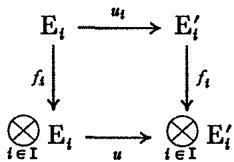
\includegraphics[keepaspectratio]{images/part003_14ac730d.jpg}}

is commutative, \(f_{i}\) and \(f_{i}^{\prime}\) denoting the canonical homomorphisms.

It suffices to apply Proposition 8 to the homomorphism \(f_{i}^{\prime} \circ u_{i}\) .

The homomorphism \(u\) defined in the Corollary to Proposition 8 is denoted by \(\bigotimes_{i \in I} u_i\) . If \(J\) is any subset of \(I\) , Proposition 8 can be applied to the family \((f_i)_{i \in J}\) of canonical homomorphisms \(f_i: E_i \to \bigotimes_{i \in I} E_i = E\) ; a canonical homomorphism \(E_J \to E\) is derived which is also denoted by \(f_J\) and which, when \(J\) is finite, coincides with the homomorphism denoted thus above.

Now let \((x_{i})_{i\in \mathbf{I}}\) be an element of \(\prod_{i\in \mathbf{I}}\mathrm{E}_i\) such that the family \((x_{i} - e_{i})_{i\in \mathbf{I}}\) has finite support H. It is immediate that, if J and \(J^{\prime}\) are two finite subsets of I containing H, then

\[
f _ {J} ((x _ {i}) _ {i \in J}) = f _ {J ^ {\prime}} ((x _ {i}) _ {i \in J ^ {\prime}}).
\]

The common value of the \(f_{\mathbf{J}}((x_i)_{i \in \mathbf{J}})\) for the finite subsets \(\mathbf{J} \supset \mathbf{H}\) of \(\mathbf{I}\) is denoted by \(\bigotimes_{i \in \mathbf{I}} x_i\) .

PROPOSITION 9. Let \((\mathbf{E}_i)_{i\in \mathbf{I}}\) be a family of A-algebras and for each \(i\in \mathbf{I}\) let \(B_{i}\) be a basis of \(\mathbf{E}_i\) such that the unit element \(e_i\) belongs to \(\overline{\mathbf{B}}_i\) . Let \(\mathbf{B}\) be the set of elements of the form \(\bigotimes_{i\in \mathbf{I}}x_i\) , where \((x_{i})\) runs through the set of elements of \(\prod_{i\in \mathbf{I}}\mathbf{B}_i\) such that the family \((x_{i} - e_{i})\) has finite support. Then \(\mathbf{B}\) is a basis of the algebra \(\bigotimes_{i\in \mathbf{I}}\mathbf{E}_i\) and this basis contains the unit element \(e\) .

For every finite subset J of I, let \(B_{J}\) be the basis of \(E_{J} = \bigotimes_{i \in J} E_{i}\) the tensor product of the bases \(B_{i}\) for \(i \in J\) (II, §3, no. 9). It follows immediately from the definitions that B is the union of the \(f_{J}(B_{J})\) when J runs through \(\mathfrak{F}(I)\) and that \(f_{J^{\prime}J}(B_{J}) \subset B_{J^{\prime}}\) when \(J \subset J^{\prime}\) ; hence \((B_{J})\) is a direct system of subsets of the \(E_{J}\) and \(B = \varinjlim B_{J}\) ; the conclusion then follows from II, §6, no. 2, Corollary to Proposition 5.

The basis B is also called the tensor product of the bases \(B_{i}\) for \(i \in I\) ; when the conditions of Proposition 9 are fulfilled, the canonical homomorphisms \(f_{J}: E_{J} \to E = \bigotimes_{i \in I} E_{i}\) are injective for every subset J of I, for if \(B_{J}\) is the basis of \(E_{J}\) the tensor product of the \(B_{i}\) for \(i \in J\) , it is immediately verified that the restriction of \(f_{J}\) to \(B_{J}\) is injective and maps \(B_{J}\) onto a subset of B.

\subsection{COMMUTATION LEMMAS}

Lemma 1. Let \(\mathbf{A}\) be a commutative ring, \(\mathbf{E}\) an \(\mathbf{A}\) -algebra, \((x_{i})_{1\leqslant i\leqslant n}\) a finite sequence of elements of \(\mathbf{E}\) , \((\lambda_i)_{1\leqslant i\leqslant n}\) a finite sequence of elements of \(\mathbf{A}\) and \(y\) an element of \(\mathbf{E}\) ; suppose that

\[
x _ {i} y = \lambda_ {i} y x _ {i} \quad \text { for } 1 \leqslant i \leqslant n.\tag{13}
\]

Then

\[
\left(x _ {1} x _ {2} \dots x _ {n}\right) y = \left(\lambda_ {1} \lambda_ {2} \dots \lambda_ {n}\right) y \left(x _ {1} x _ {2} \dots x _ {n}\right).\tag{14}
\]

The lemma being trivial for \(n = 1\) , we argue by induction on \(n \geqslant 2\) . Now

\[
\begin{array}{r l} (x _ {1} x _ {2} \dots x _ {n}) y & = (x _ {1} \dots x _ {n - 1}) (x _ {n} y) \\ & = (x _ {1} \dots x _ {n - 1}) (\lambda_ {n} y x _ {n}) = \lambda_ {n} ((x _ {1} \dots x _ {n - 1}) y) x _ {n}, \end{array}
\]

which, by the induction hypothesis, is equal to

\[
\lambda_ {n} \left(\lambda_ {1} \dots \lambda_ {n - 1}\right) y \left(x _ {1} \dots x _ {n - 1}\right) x _ {n} = \left(\lambda_ {1} \dots \lambda_ {n - 1} \lambda_ {n}\right) y \left(x _ {1} \dots x _ {n - 1} x _ {n}\right),
\]

whence the lemma.

Lemma 2. Let A be a commutative ring, E an A-algebra and \((x_{i})_{1\leqslant i\leqslant n}\) and \((y_{i})_{1\leqslant i\leqslant n}\) two finite sequences of \(n\) elements of E; suppose that for \(1\leqslant j\leqslant i\leqslant n\) ,

\[
x _ {i} y _ {j} = \lambda_ {i j} y _ {j} x _ {i} \quad \text { with } \lambda_ {i j} \in A.\tag{15}
\]

Then

\[
\left(x _ {1} x _ {2} \dots x _ {n}\right) \left(y _ {1} y _ {2} \dots y _ {n}\right) = \left(\prod_ {i > j} \lambda_ {i j}\right) \left(x _ {1} y _ {1}\right) \left(x _ {2} y _ {2}\right) \dots \left(x _ {n} y _ {n}\right).\tag{16}
\]

The lemma being trivial for \(n = 1\) , we again argue by induction on \(n\) for \(n \geqslant 2\) . By virtue of Lemma 1,

\[
\begin{array}{r l} (x _ {1} \dots x _ {n}) (y _ {1} \dots y _ {n}) & = x _ {1} (x _ {2} \dots x _ {n}) y _ {1} (y _ {2} \dots y _ {n}) \\ & = \left(\prod_ {i > 1} \lambda_ {i 1}\right) (x _ {1} y _ {1}) (x _ {2} \dots x _ {n}) (y _ {2} \dots y _ {n}) \end{array}
\]

and it then suffices to apply the induction hypothesis to obtain (16).

For every family \(\lambda = (\lambda_{ij})\) of elements of A, with \(1 \leqslant j < i \leqslant n\) , and for every permutation \(\sigma \in \mathfrak{S}_n\) , we write

\[
\varepsilon_ {\sigma} (\lambda) = \prod_ {i > j, \sigma^ {- 1} (i) < \sigma^ {- 1} (j)} \lambda_ {i j} = \prod_ {i <   j, \sigma (i) > \sigma (j)} \lambda_ {\sigma (i), \sigma (j)}.\tag{17}
\]

Observe that, when \(\mathbf{A} = \mathbf{Z}\) and \(\lambda_{ij} = -1\) for every ordered pair \((i,j)\) such that \(1 \leqslant j < i \leqslant n\) , \(\varepsilon_{\sigma}(\lambda)\) is just the signature \(\varepsilon_{\sigma}\) of the permutation \(\sigma\) (I, § 5, no. 7).

Lemma 3. Let A be a commutative ring, E an A-algebra, \((x_{i})_{1\leqslant i\leqslant n}\) a finite sequence of elements of E and suppose that, for every ordered pair \((i,j)\) of integers such that \(1\leqslant j < i\leqslant n\) ,

\[
x _ {i} x _ {j} = \lambda_ {i j} x _ {j} x _ {i} \quad \text { with } \lambda_ {i j} \in A.\tag{18}
\]

Then, for every permutation \(\sigma \in \mathfrak{S}_n\) ,

\[
x _ {\sigma (1)} x _ {\sigma (2)} \dots x _ {\sigma (n)} = \varepsilon_ {\sigma} (\lambda) x _ {1} x _ {2} \dots x _ {n}.\tag{19}
\]

The lemma is trivial for \(n = 1\) and \(n = 2\) ; we proceed by induction on \(n\) for \(n \geqslant 3\) . If \(\sigma(n) = n\) , relation (19) follows from the induction hypothesis. Suppose therefore that \(\sigma(n) = k, k \neq n\) , and let \(\tau\) be the permutation of \([1, n]\) defined by

\[
\left\{ \begin{array}{l l} \tau (i) = i & \text { for } i <   k \\ \tau (i) = i + 1 & \text { for } k \leqslant i <   n \\ \tau (n) = k. \end{array} \right.
\]

Let \(\pi = \tau^{-1} \circ \sigma\) ; the permutation \(\pi\) leaves \(n\) fixed; now \(\sigma = \tau \circ \pi\) and therefore, writing \(y_i = x_{\tau(i)}\) , \(y_{\pi(i)} = x_{\sigma(i)}\) . If \(i \neq n\) and \(j \neq n\) , the relations \(\pi(i) > \pi(j)\) and \(\sigma(i) > \sigma(j)\) are equivalent (since \(\tau\) is a strictly increasing mapping of \([1, n - 1]\) into \([1, n]\) . For \(i \neq n\) , \(j \neq n\) and \(\sigma(i) > \sigma(j)\) ,

\[
y _ {\pi (i)} y _ {\pi (j)} = x _ {\sigma (i)} x _ {\sigma (j)} = \lambda_ {\sigma (i), \sigma (j)} x _ {\sigma (j)} x _ {\sigma (i)} = \lambda_ {\sigma (i), \sigma (j)} y _ {\pi (j)} y _ {\pi (i)}
\]

whence, by the induction hypothesis (using the fact that \(\pi(n) = n\) ):

\[
y _ {\pi (1)} y _ {\pi (2)} \dots y _ {\pi (n)} = \left(\prod_ {i <   j <   n, \sigma (i) > \sigma (j)} \lambda_ {\sigma (i), \sigma (j)}\right) y _ {1} y _ {2} \dots y _ {n}
\]

that is

\[
x _ {\sigma (1)} x _ {\sigma (2)} \dots x _ {\sigma (n)} = \left(\prod_ {i <   j <   n, \sigma (i) > \sigma (j)} \lambda_ {\sigma (i), \sigma (j)}\right) x _ {\tau (1)} \dots x _ {\tau (n)}.\tag{20}
\]

Now

\[
x _ {\tau (1)} \dots x _ {\tau (n)} = x _ {1} \dots x _ {k - 1} x _ {k + 1} \dots x _ {n} x _ {k}
\]

and this, by Lemma 1, is equal to

\[
\left(\prod_ {j > k} \lambda_ {j k}\right) x _ {1} \dots x _ {n} = \left(\prod_ {\sigma (i) > \sigma (n)} \lambda_ {\sigma (i), \sigma (n)}\right) x _ {1} \dots x _ {n}.\tag{21}
\]

Finally, (20) and (21) give

\[
x _ {\sigma (1)} \dots x _ {\sigma (n)} = \alpha . x _ {1} \dots x _ {n}
\]

with

\[
\begin{array}{l} \alpha = \left(\prod_ {i <   j <   n, \sigma (i) > \sigma (j)} \lambda_ {\sigma (i), \sigma (j)}\right) \cdot \left(\prod_ {i <   n, \sigma (i) > \sigma (n)} \lambda_ {\sigma (i), \sigma (n)}\right) \\ = \prod_ {i <   j, \sigma (i) > \sigma (j)} \lambda_ {\sigma (i), \sigma (j)} = \varepsilon_ {\sigma} (\lambda) \end{array}
\]

which completes the proof of Lemma 3.

\subsection{TENSOR PRODUCT OF GRADED ALGEBRAS RELATIVE TO COMMUTATION FACTORS}

DEFINITION 6. Let \((\Delta_{i})_{i\in I}\) be a finite family of commutative monoids written additively. A system of commutation factors over the \(\Delta_{i}\) with values in a commutative ring A is a system of mappings \(\varepsilon_{ij}:\Delta_i\times \Delta_j\to \mathbf{A}\) , where \(i\in \mathbf{I}, j\in \mathbf{I}, i\neq j\) satisfying the following conditions:

\[
\varepsilon_ {i j} \left(\alpha_ {i} + \alpha_ {i} ^ {\prime}, \beta_ {j}\right) = \varepsilon_ {i j} \left(\alpha_ {i}, \beta_ {j}\right) \varepsilon_ {i j} \left(\alpha_ {i} ^ {\prime}, \beta_ {j}\right)\tag{22}
\]

\[
\varepsilon_ {i j} \left(\alpha_ {i}, \beta_ {j} + \beta_ {j} ^ {\prime}\right) = \varepsilon_ {i j} \left(\alpha_ {i}, \beta_ {j}\right) \varepsilon_ {i j} \left(\alpha_ {i}, \beta_ {j} ^ {\prime}\right)\tag{23}
\]

\[
\varepsilon_ {i j} (\alpha_ {i}, \beta_ {j}) \varepsilon_ {j i} (\beta_ {j}, \alpha_ {i}) = 1,\tag{24}
\]

for all \(\alpha_{i},\alpha_{i}^{\prime}\) in \(\Delta_{i},\beta_{j},\beta_{j}^{\prime}\) in \(\Delta_j\).

If I is given a total ordering and the \(\Delta_{i}\) are groups, a system of commutation factors is defined over the \(\Delta_{i}\) by taking for every ordered pair \((i,j)\) such that i\textless j an arbitrary Z-bilinear mapping of \(\Delta_{i}\times\Delta_{j}\) into the (multiplicative) Z-module A* of invertible elements of the ring A and then writing

\[
\varepsilon_ {j i} (\beta_ {j}, \alpha_ {i}) = (\varepsilon_ {i j} (\alpha_ {i}, \beta_ {j})) ^ {- 1}
\]

for \(i < j\) .

Note that, since the \(\varepsilon_{ij}(\alpha_{i},\beta_{j})\) are invertible,

\[
\varepsilon_ {i j} (0, \beta_ {j}) = \varepsilon_ {i j} (\alpha_ {i}, 0) = 1,
\]

by virtue of (22) and (23).

Examples. (1) The trivial system of commutation factors consists of the \(\varepsilon_{ij}\) such that \(\varepsilon_{ij}(\alpha_i, \beta_j) = 1\) for all \(i, j, \alpha_i \in \Delta_i, \beta_j \in \Delta_j\) .

\begin{enumerate}
\def\labelenumi{(\arabic{enumi})}
\setcounter{enumi}{1}
\tightlist
\item
  If we take \(\mathbf{A} = \mathbf{Z}\) and \(\Delta_{i} = \mathbf{Z}\) for all \(i \in \mathbf{I}\) , a system of commutation factors is obtained by taking \(\varepsilon_{ij}(\alpha_i, \beta_j) = (-1)^{\alpha_i\beta_j}\) . Note that this number depends only on the parities of \(\alpha_{i}\) and \(\beta_{j}\) and the \(\varepsilon_{ij}\) can therefore be considered as commutation factors when certain of the \(\Delta_{i}\) are equal to \(\mathbf{Z}/2\mathbf{Z}\) and the others to \(\mathbf{Z}\) .
\end{enumerate}

These two examples are the most frequent cases encountered in applications.

PROPOSITION 10. Let A be a commutative ring and \((\Delta_{i})_{i\in I}\) a finite family of commutative monoids written additively; for each \(i\in I\) let \(\mathbf{E}_i\) be a graded A-algebra of type \(\Delta_i\) . Finally, let \((\varepsilon_{ij})\) be a system of commutation factors over the \(\Delta_i\) with values in A. Then there exist a graded A-algebra E of type \(\Delta = \prod_{i\in I}\Delta_i\) and for each \(i\in I\) an algebra homomorphism \(h_i:\mathbf{E}_i\to \mathbf{E}\) , with the following properties:

\begin{enumerate}
\def\labelenumi{(\roman{enumi})}
\item
  If \(\phi_{i}:\Delta_{i}\to\Delta\) is the canonical homomorphism, then \(h_{i}\) is a graded homomorphism (II, § 11, no. 2), in other words, \(h_{i}(E_{i}^{\alpha_{i}})\subset E^{\phi_{i}(\alpha_{i})}\) , where \((E_{i}^{\alpha_{i}})\) and \((E^{\alpha})\) denote the respective graduations on \(E_{i}\) and \(E\) .
\item
  If \(i \neq j\) and \(x_{i}\) (resp. \(x_{j}\) ) is a homogeneous element of \(\mathbf{E}_i\) (resp. \(\mathbf{E}_j\) ) of degree \(\alpha_i \in \Delta_i\) (resp. \(\beta_j \in \Delta_j\) ), then
\end{enumerate}

\[
h _ {i} (x _ {i}) h _ {j} (x _ {j}) = \varepsilon_ {i j} (\alpha_ {i}, \beta_ {j}) h _ {j} (x _ {j}) h _ {i} (x _ {i}).\tag{25}
\]

\begin{enumerate}
\def\labelenumi{(\roman{enumi})}
\setcounter{enumi}{2}
\tightlist
\item
  For every A-algebra \(\mathbf{F}\) and every system of homomorphisms \(f_{i}:\mathbf{E}_{i}\to \mathbf{F}\) satisfying the conditions
\end{enumerate}

\[
f _ {i} (x _ {i}) f _ {j} (x _ {j}) = \varepsilon_ {i j} (\alpha_ {i}, \beta_ {j}) f _ {j} (x _ {j}) f _ {i} (x _ {i}),\tag{26}
\]

where \(i, j, x_i, x_j, \alpha_i, \beta_j\) are as in (ii), then there exists one and only one algebra homomorphism \(f: \mathbf{E} \to \mathbf{F}\) such that \(f_i = f \circ h_i\) for all \(i \in \mathbf{I}\) . Moreover the underlying A-module of \(\mathbf{E}\) is the tensor product \(\bigotimes_{i \in \mathbf{I}} \mathbf{E}_i\) .

Consider the A-module \(E = \bigotimes_{i \in I} E_i\) ; it is identified with the direct sum of the submodules \(E^\alpha\) , where, for each \(\alpha = (\alpha_i) \in \Delta\) , we write \(E^\alpha = \bigotimes_{i \in I} E_i^{\alpha_i}\) ; the \(E^\alpha\) therefore form a graduation of type \(\Delta\) on the A-module E. We shall define on E a graded A-algebra structure of type \(\Delta\) . For this let I be given a total ordering; for every ordered pair of elements \(\alpha = (\alpha_i)\) , \(\beta = (\beta_i)\) of \(\Delta\) , we must first define an A-bilinear mapping of \(E^\alpha \times E^\beta\) into \(E^\alpha + \beta\) , or alternatively an A-linear mapping \(m_{\alpha\beta}\) of \(E^\alpha \otimes_A E^\beta\) into \(E^\alpha + \beta\) . We shall define \(m_{\alpha\beta}\) by the condition

\[
m _ {\alpha \beta} \left(\left(\bigotimes_ {i \in I} x _ {i}\right) \otimes \left(\bigotimes_ {i \in I} y _ {i}\right)\right) = \varepsilon (\alpha , \beta) \bigotimes_ {i \in I} (x _ {i} y _ {i})\tag{27}
\]

for \(x_{i}\in \mathrm{E}_{i}^{\alpha_{i}},y_{i}\in \mathrm{E}_{i}^{\beta_{i}}\) , where

\[
\varepsilon (\alpha , \beta) = \prod_ {i > j} \varepsilon_ {i j} (\alpha_ {i}, \beta_ {j}).\tag{28}
\]

The right hand side of (27) obviously belongs to \(\mathbf{E}^{\alpha +\beta}\) and the mapping \((x_{1},\ldots ,x_{n},y_{1},\ldots ,y_{n})\mapsto \varepsilon (\alpha ,\beta)\bigotimes_{i\in I}(x_{i}y_{i})\) is A-multilinear in the product of the \(\mathrm{E}_i^{\alpha_i}\) and the \(\mathrm{E}_i^{\beta_i}(1\leqslant i\leqslant n)\) . Then it must be proved that the multiplication thus defined on E is associative; now, if \(\gamma = (\gamma_{i})\) is a third element of \(\Delta\) and \(z_{i} \in \mathrm{E}_{i}^{\gamma_{i}}\) for \(1 \leqslant i \leqslant n\) , then

\[
\left(\left(\bigotimes_ {i} x _ {i}\right) \left(\bigotimes_ {i} y _ {i}\right)\right) \left(\bigotimes_ {i} z _ {i}\right) = \varepsilon (\alpha + \beta , \gamma) \varepsilon (\alpha , \beta) \bigotimes_ {i} (x _ {i} y _ {i} z _ {i})
\]

\[
\left(\bigotimes_ {i} x _ {i}\right) \left(\left(\bigotimes_ {i} y _ {i}\right) \left(\bigotimes_ {i} z _ {i}\right)\right) = \varepsilon (\alpha , \beta + \gamma) \varepsilon (\beta , \gamma) \bigotimes_ {i} (x _ {i} y _ {i} z _ {i})
\]

and it reduces to verifying the identity

\[
\varepsilon (\alpha + \beta , \gamma) \varepsilon (\alpha , \beta) = \varepsilon (\alpha , \beta + \gamma) \varepsilon (\beta , \gamma).
\]

But the latter follows immediately from the relations

\[
\varepsilon (\alpha + \beta , \gamma) = \varepsilon (\alpha , \beta) \varepsilon (\beta , \gamma)
\]

\[
\varepsilon (\alpha , \beta + \gamma) = \varepsilon (\alpha , \beta) \varepsilon (\alpha , \gamma)
\]

themselves immediate consequences of the definition (28) and (22) and (23).

If, for all \(i \in \mathbf{I}\) , \(e_i\) denotes the unit element of \(\mathbf{E}_i\) , we know that \(e_i\) is homogeneous of degree 0 (§ 3, no. 1), hence \(e = \bigotimes_{i \in \mathbf{I}} e_i\) is homogeneous of degree 0 and it follows from (27), (28) and the relations

\[
\varepsilon_ {i j} (\alpha_ {i}, 0) = \varepsilon_ {i j} (0, \beta_ {j}) = 1
\]

that \(e\) is unit element of \(\mathbf{E}\) , which completes the definition on \(\mathbf{E}\) of the desired graded A-algebra structure. Then take \(h_i(x_i) = x_i \otimes \bigotimes_{j \neq i} e_j\) ; to verify that \(h_i(x_i x_i') = h_i(x_i) h_i(x_i')\) for \(x_i, x_i'\) in \(\mathbf{E}_i\) , attention may be confined to the case where \(x_i\) and \(x_i'\) are homogeneous and then this relation follows immediately from (27) and the relations \(\varepsilon_{ij}(\alpha_i, 0) = \varepsilon_{ij}(0, \beta_j) = 1\) ; the same relations and (24) prove also that the \(h_i\) satisfy conditions (i) and (ii) of the statement and that

\[
\bigotimes_ {i \in I} x _ {i} = \prod_ {i \in I} h _ {i} (x _ {i})\tag{29}
\]

where the right hand side is the product of the ordered sequence \((h_i(x_i))_{i\in I}\) in E with the given total ordering on I (I, § 1, no. 2) (it suffices to argue by induction on the number of \(x_{i}\) (assumed homogeneous) distinct from the \(e_i\) ).

It remains to prove condition (iii); note that the mapping

\[
(x _ {i}) _ {i \in I} \mapsto \prod_ {i \in I} f _ {i} (x _ {i}),
\]

where the right hand side is the product of the ordered sequence \((f_{i}(x_{i}))_{i\in\mathbf{I}}\) with the given total ordering on I, is A-multilinear. Then there exists one and only one A-linear mapping \(f: E \rightarrow F\) such that

\[
f \left(\bigotimes_ {i \in I} x _ {i}\right) = \prod_ {i \in I} f _ {i} (x _ {i}).\tag{30}
\]

Clearly \(f(e)\) is the unit element of \(\mathbf{F}\) and \(f \circ h_i = f_i\) ; to verify that \(f\) is an algebra homomorphism, in other words that \(f(x)f(y) = f(xy)\) for \(x, y\) in \(\mathbf{E}\) , attention may be confined, by linearity, to the case where \(x = \bigotimes_{i \in \mathbf{I}} x_i\) and \(y = \bigotimes_{i \in \mathbf{I}} y_i\) , \(x_i\) (resp. \(y_i\) ) being homogeneous of degree \(\alpha_i\) (resp. \(\beta_i\) ) for all \(i \in \mathbf{I}\) . The relation to be verified then reduces, by (27), to

\[
\left(\prod_ {i \in \mathrm{I}} f _ {i} (x _ {i})\right) \left(\prod_ {i \in \mathrm{I}} f _ {i} (y _ {i})\right) = \varepsilon (\alpha , \beta) \prod_ {i \in \mathrm{I}} \left(f _ {i} (x _ {i}) f _ {i} (y _ {i})\right).
\]

But, taking account of relations (26), this is a consequence of Lemma 2 of no. 6.

Clearly the algebra E and the canonical mapping \(\psi: \bigotimes_{i \in I} E_i \to E\) constitute a solution of the universal mapping problem (Set Theory, IV, § 3, no. 1), where \(\Sigma\) is the species of A-algebra structure and the \(\alpha\) -mappings \(\prod_{i} f_i\) from \(\prod_{i} E_i\) to an A-algebra, satisfying conditions (26).

For a fixed total ordering on I, the graded algebra E defined in the proof of Proposition 10 will be called a graded tensor \(\varepsilon\) -product of type \(\Delta\) of the family \((\mathrm{E}_i)_{i\in \mathbf{I}}\) of graded algebras of type \(\Delta_i\) and will be denoted by \({}^{\varepsilon}\bigotimes_{i\in \mathbf{I}}\mathrm{E}_i\) (if no confusion can arise over the ordering on I); similarly, the homomorphism \(f:\mathrm{E}\to \mathrm{F}\) defined in the proof of Proposition 10 will be denoted by \({}^{\varepsilon}\bigotimes_{i\in \mathbf{I}}f_i\) . The homomorphisms \(h_i\) are called canonical. We also write \({}^{\varepsilon}\mathrm{G}^{\otimes n}\) when \(\mathbf{I} = [1,n]\) and all the \(\mathrm{E}_i\) are equal to the same algebra G.

Remarks. (1) We recover the tensor product of algebras defined in no. 1 (with moreover the graduation the tensor product of those of its factors) taking \(\varepsilon_{ij}(\alpha_i, \beta_j) = 1\) for all \(i, j, \alpha_i\) and \(\beta_j\) .

\begin{enumerate}
\def\labelenumi{(\arabic{enumi})}
\setcounter{enumi}{1}
\tightlist
\item
  Suppose that all the \(\Delta_{i}\) are equal to \(\mathbf{Z}\) and write \(\varepsilon_{ij}(\alpha_i, \beta_j) = (-1)^{\alpha_i \beta_j}\) ; the tensor \(\varepsilon\) -product \({}^{\varepsilon}\bigotimes_{i \in I} E_i\) corresponding to this system of commutation factors is then called the skew tensor product of the graded algebras \(E_i\) of type \(\mathbf{Z}\) and denoted by \({}^{g}\bigotimes_{i \in I} E_i\) (or \(E{}^{g} \otimes_A F\) for two algebras, or \({}^{g} G^{\otimes n}\) instead of \({}^{\varepsilon} G^{\otimes n}\) ).
\end{enumerate}

COROLLARY 1. In the notation of Proposition 10, suppose further that F is a graded A-algebra of type \(\Delta\) and that each \(f_{i}\) is a graded algebra homomorphism relative to \(\phi_{i}:\Delta_{i}\to\Delta\) ; then \(f={}^{\varepsilon}\bigotimes_{i}f_{i}\) is a graded algebra homomorphism.

This follows immediately from the definition of \(f\) and the fact that

\[
\sum_ {i \in I} \phi_ {i} (\alpha_ {i}) = (\alpha_ {i})
\]

by definition of the \(\phi_{i}\) .

It is therefore seen that \((\mathrm{E},\psi)\) is also a solution of another universal mapping problem, where this time \(\Sigma\) is the species of graded A-algebra structure of type \(\Delta\) , the morphisms being graded algebra homomorphisms of type \(\Delta\) and the \(\alpha\) -mappings the mappings \(\prod_{i}f_{i}\) , where, in addition to conditions (26), it is assumed that \(f_{i}\) is a graded algebra homomorphism relative to \(\phi_{i}\) .

COROLLARY 2. Let \((\mathbf{E}_i)_{i\in \mathbf{I}}\) , \((\mathbf{F}_i)_{i\in \mathbf{I}}\) be two finite families of A-algebras, with \(\mathbf{E}_i\) and \(\mathbf{F}_i\) graded of type \(\Delta_i\) for all \(i\in \mathbf{I}\) . For each \(i\in \mathbf{I}\) , let \(g_i:\mathbf{E}_i\to \mathbf{F}_i\) be a graded algebra homomorphism of type \(\Delta_i\) . Then, if \(h_i:\mathbf{E}_i\to {}^{\varepsilon}\bigotimes_{i\in \mathbf{I}}\mathbf{E}_i\) and \(h_i':\mathbf{F}_i\to {}^{\varepsilon}\bigotimes_{i\in \mathbf{I}}\mathbf{F}_i\) are the canonical homomorphisms, there exists one and only one homomorphism of graded A-algebras of type \(\Delta\) , \(g: {}^{\varepsilon}\bigotimes_{i\in \mathbf{I}}\mathbf{E}_i\to {}^{\varepsilon}\bigotimes_{i\in \mathbf{I}}\mathbf{F}_i\) such that \(g\circ h_i = h_i'\circ g_i\) for all \(i\in \mathbf{I}\) . Also, if each \(g_i\) is bijective, so is \(g\) .

It suffices to apply Corollary 1 to \(f_{i} = h_{i}^{\prime} \circ g_{i}\) , noting that conditions (26) then follow from relations (25) applied to the \(h_{i}^{\prime}\) .

The homomorphism defined in Corollary 2 is also denoted by \({}^{\varepsilon}\bigotimes_{i} g_{i}\) (if no confusion can arise); if, for each \(i \in I\) , \(G_{i}\) is a third graded A-algebra of type \(\Delta_{i}\) and \(g_{i}^{\prime}: F_{i} \to G_{i}\) a graded algebra homomorphism, then

\[
\left(^ {\varepsilon} \bigotimes_ {i} g _ {i} ^ {\prime}\right) \circ \left(^ {\varepsilon} \bigotimes_ {i} g _ {i}\right) = ^ {\varepsilon} \bigotimes_ {i} \left(g _ {i} ^ {\prime} \circ g _ {i}\right),\tag{31}
\]

as follows immediately from (30).

In the case of a skew tensor product of graded algebras of type \(\mathbf{Z}\) , we write \({}^{g}\bigotimes_{i}f_{i}\) instead of \({}^{\varepsilon}\bigotimes_{i}f_{i}\) for homomorphisms \(f_{i}: \mathrm{E}_{i} \to \mathrm{F}_{i}\) of graded algebras of type \(\mathbf{Z}\) ; when \(\mathrm{I} = \{1, 2\}\) , this homomorphism is also denoted by \(f_{1}{}^{g}\otimes f_{2}\) ; when \(\mathrm{I} = [1, n]\) and all the \(\mathrm{E}_{i}\) (resp. \(\mathrm{F}_{i}\) ) are equal and all the \(f_{i}\) equal to the same homomorphism \(f\) , we write \({}^{g}f^{\otimes n}\) .

Remark. In the proof of Proposition 10, a total ordering on I was used to define an algebra structure on the tensor product \(\bigotimes_{i\in I}E_i\) of the A-modules

\(E_{i}\) . If the ordering on I is changed, another multiplicative structure arises on \(\bigotimes_{i\in I}E_{i}\) , but the new algebra thus obtained is canonically isomorphic to the above, since both are solutions of the same universal mapping problem. For example, when \(I=\{1,2\}\) , the canonical isomorphism of the algebra \(E_{1}{}^{\varepsilon}\otimes_{A}E_{2}\) onto the algebra \(E_{2}{}^{\varepsilon}\otimes_{A}E_{1}\) maps \(x_{1}\otimes x_{2}\) to \(\varepsilon_{2,1}(\alpha,\beta)x_{2}\otimes x_{1}\) , where \(x_{1}\) is homogeneous of degree \(\alpha\) and \(x_{2}\) homogeneous of degree \(\beta\) .

Let J be a subset of I and, for each \(i \in J\) , consider the canonical homomorphism \(h_{i}: E_{i} \to {}^{\varepsilon}\bigotimes_{i \in I} E_{i} = E\) . By virtue of relations (25) a canonical homomorphism \(h: E' = {}^{\varepsilon}\bigotimes_{i \in J} E_{i} \to E\) is derived canonically (by Proposition 10) from these homomorphisms, such that, for all \(i \in J\) , \(h_{i}' = h \circ h_{i}\) , \(h_{i}'\) being the canonical homomorphism \(E_{i} \to E'\) . Taking the total ordering on J induced by that chosen on I, we obtain

\[
h \left(\bigotimes_ {i \in J} x _ {i}\right) = \prod_ {i \in I} h _ {i} \left(x _ {i}\right) = \bigotimes_ {i \in I} x _ {i} ^ {\prime}
\]

where the middle term is the product of the ordered sequence \((h_i(x_i))_{i\in J}\) and where, in the right hand term, \(x_{i}^{\prime} = x_{i}\) for \(i\in J\) , \(x_{i}^{\prime} = e_{i}\) for \(i\notin J\) .

PROPOSITION 11. (``associativity'' of the tensor \(\varepsilon\) -product). In the notation of Proposition 10, let \((J_{\lambda})_{\lambda \in L}\) be a partition of I and write \(\Delta_{\lambda}' = \prod_{i \in J_{\lambda}} \Delta_i\) for all \(\lambda \in L\) . Let \(E_{\lambda}'\) be a graded tensor \(\varepsilon\) -product of type \(\Delta_{\lambda}'\) of the family \((E_i)_{i \in J_{\lambda}}\) (for some total ordering chosen on \(J_{\lambda}\) ). On the other hand, for \(\lambda, \mu\) in L and \(\lambda \neq \mu\) , we write, for \(\alpha_{\lambda}' = (\alpha_i)_{i \in J_{\lambda}}, \beta_{\mu}' = (\beta_j)_{j \in J_{\mu}}\) ,

\[
\varepsilon_ {\lambda \mu} ^ {\prime} (\alpha _ {\lambda} ^ {\prime}, \beta_ {\mu} ^ {\prime}) = \prod_ {i \in J _ {\lambda}, j \in J _ {\mu}} \varepsilon_ {i j} (\alpha_ {i}, \beta_ {j}).\tag{32}
\]

Then \((\varepsilon_{\lambda \mu}^{\prime})\) is a system of commutation factors over the \(\Delta_{\lambda}^{\prime}\) with values in A and there exists one and only one homomorphism of graded algebras of type \(\Delta, v: {}^{\varepsilon'}\bigotimes_{\lambda \in L} E_{\lambda}^{\prime} \to {}^{\varepsilon}\bigotimes_{i \in I} E_{i}\) , such that

\[
v \left(\bigotimes_ {\lambda \in L} \left(\bigotimes_ {i \in J _ {\lambda}} x _ {i}\right)\right) = \bigotimes_ {i \in I} x _ {i}\tag{33}
\]

for all \((x_{i})\in \prod_{i\in \mathbf{I}}\mathrm{E}_{i}\) , provided that the total ordering is taken on \(\mathbf{I}\) which induces on each \(\mathbf{J}_{\lambda}\) the chosen total ordering, and which is such that, for \(\lambda < \mu\) in \(\mathbf{L}\) , \(i\in \mathbf{J}_{\lambda}\) and \(j\in \mathbf{J}_{\mu}\) , \(i < j\) .

The fact that the \(\varepsilon_{\lambda \mu}'\) form a system of commutation factors is trivial. Let \(h_{i,\lambda}:\mathrm{E}_i\to \mathrm{E}_{\lambda}', h_{\lambda}':\mathrm{E}_{\lambda}'\to {}^{\varepsilon'}\bigotimes_{\lambda \in L}\mathrm{E}_{\lambda}'\) be the canonical homomorphisms (for \(\lambda \in L\) , \(i\in \mathbf{J}_{\lambda}\) ) and write \(h_i'' = h_\lambda' \circ h_{i,\lambda}\) ; it will suffice by virtue of the uniqueness of the solution of a universal mapping problem, to show that \({}^{\varepsilon'}\bigotimes_{\lambda \in L} E_{\lambda}'\) and the \(h_i''\) satisfy the conditions of Proposition 10. Now, for all \(\lambda \in L\) , let \(f_{\lambda}': E_{\lambda}' \to F\) be the unique algebra homomorphism such that \(f_{\lambda}' \circ h_{i,\lambda} = f_i\) for all \(i \in J_{\lambda}\) . We show that, for \(\lambda \neq \mu\) , \(\alpha_{\lambda}' = (\alpha_i)_{i \in J_{\lambda}}\) , \(\beta_{\mu}' = (\beta_j)_{j \in J_{\mu}}\) ,

\[
f _ {\lambda} ^ {\prime} (x _ {\lambda} ^ {\prime}) f _ {\mu} ^ {\prime} (x _ {\mu} ^ {\prime}) = \varepsilon_ {\lambda \mu} ^ {\prime} (\alpha_ {\lambda} ^ {\prime}, \beta_ {\mu} ^ {\prime}) f _ {\mu} ^ {\prime} (x _ {\mu} ^ {\prime}) f _ {\lambda} ^ {\prime} (x _ {\lambda} ^ {\prime})\tag{34}
\]

for \(x_{\lambda}^{\prime} \in \mathrm{E}_{\lambda}^{\prime}\) (resp. \(x_{\mu}^{\prime} \in \mathrm{E}_{\mu}^{\prime}\) ) homogeneous of degree \(\alpha_{\lambda}^{\prime}\) (resp. \(\beta_{\mu}^{\prime}\) ); it suffices, by linearity, to verify it when \(x_{\lambda}^{\prime} = \bigotimes_{i \in J_{\lambda}} x_{i}\) , \(x_{\mu}^{\prime} = \bigotimes_{j \in J_{\mu}} x_{j}\) , \(x_{i}\) (resp. \(x_{j}\) ) being homogeneous of degree \(\alpha_{i}\) (resp. \(\beta_{j}\) ) in \(E_{i}\) (resp. \(E_{j}\) ) for \(i \in J_{\lambda}, j \in J_{\mu}\) . But this follows from formula (30) which defines the \(f_{\lambda}^{\prime}\) and Lemma 3 of no. 6, taking account of hypothesis (26) and definition (32). There is therefore one and only one algebra homomorphism \(f: ^{\varepsilon'} \bigotimes_{\lambda \in L} E_{\lambda}' \to F\) such that \(f \circ h_{\lambda}' = f_{\lambda}'\) for all \(\lambda \in L\) ; whence \(f \circ h_{i}' = f_{i}\) for all \(i \in I\) and the uniqueness of \(f\) is trivial.

\subsection{TENSOR PRODUCT OF GRADED ALGEBRAS OF THE SAME TYPES}

Assuming the hypotheses of no. 7, Proposition 10 hold, suppose further that all the \(\Delta_{i}\) are equal to the same commutative monoid \(\Delta_{0}\) ; we can then consider on the tensor \(\varepsilon\) -product \({}^{\varepsilon}\bigotimes_{i\in I}E_{i}\) the total graduation of type \(\Delta_{0}\) , associated with the graduation of type \(\Delta = \Delta_{0}^{I}\) on this algebra (II, § 11, no. 1); we shall call \({}^{\varepsilon}\bigotimes_{i\in I}E_{i}\) , with this graduation, a graded tensor \(\varepsilon\) -product of type \(\Delta_{0}\) of the family \((E_{i})_{i\in I}\) of graded algebras of type \(\Delta_{0}\) .

Always preserving the notation of Proposition 10 of no. 7, suppose that F is also a graded A-algebra of type \(\Delta_0\) and that the \(f_i\) are homomorphisms of graded algebras of type \(\Delta_0\) . Then \(f: {}^{\varepsilon}\bigotimes_{i \in I} E_i \to F\) is also a homomorphism of graded algebras of type \(\Delta_0\) : for it follows from formula (30) (no. 7) that if \(x_i\) is homogeneous and of degree \(\alpha_i \in \Delta_0\) , \(\bigotimes_{i \in I} x_i\) and \(\prod_{i \in I} f_i(x_i)\) are both homogeneous of degree \(\sum_{i \in I} \alpha_i \in \Delta_0\) .

It can therefore be said that \(\bigotimes_{i\in I}E_i\) , with the total graduation of type \(\Delta_0\) , constitutes, together with the canonical mapping \(\psi\) , a solution of a third universal mapping problem, where \(\Sigma\) is the species of graded A-algebra of type \(\Delta_0\) , the morphisms are homomorphisms of graded algebras of type \(\Delta_0\) and the \(\alpha\) -mappings are the mappings \(\prod_{i}f_{i}\) , where, in addition to conditions (26) (of no. 7), it is assumed that each \(f_{i}\) is a homomorphism of graded algebras of type \(\Delta_0\) .

For every subset J of I, the canonical homomorphism \({}^{\varepsilon}\bigotimes_{i\in J}E_i\to {}^{\varepsilon}\bigotimes_{i\in I}E_i\) (no. 7) is, in fact, a homomorphism of graded algebras of type \(\Delta_0\) , as follows immediately from the above.

PROPOSITION 12. (``associativity'' of the tensor \(\varepsilon\) -product of graded algebras of the same types). With the notation of Proposition 10 of no. 7, suppose that all the \(\Delta_{i}\) are equal to the same monoid \(\Delta_{0}\) ; let \((J_{\lambda})_{\lambda \in L}\) be a partition of I. With the notation of Proposition 11 of no. 7, suppose that the right hand side of formula (32) (no. 7) depends only on the sums \(\alpha_{\lambda}^{\prime \prime} = \sum_{i \in J_{\lambda}} \alpha_{i}, \beta_{\mu}^{\prime \prime} = \sum_{j \in J_{\mu}} \beta_{j}\) , for every ordered pair \((\lambda, \mu)\) of distinct indices, all \(\alpha_{\lambda}^{\prime} \in \Delta_{\lambda}^{\prime}\) and all \(\beta_{\mu}^{\prime} \in \Delta_{\mu}^{\prime}\) ; let \(\varepsilon_{\lambda \mu}^{\prime \prime}(\alpha_{\lambda}^{\prime \prime}, \beta_{\mu}^{\prime \prime})\) denote the right hand side of (32). Then \((\varepsilon_{\lambda \mu}^{\prime \prime})\) is a system of commutation factors over the family \((\Delta_{\lambda}^{\prime \prime})_{\lambda \in L}\) , where \(\Delta_{\lambda}^{\prime \prime} = \Delta_{0}\) for all \(\lambda \in L\) . If \(E_{\lambda}^{\prime \prime}\) is the graded tensor \(\varepsilon\) -product of type \(\Delta_{0}\) of the family \((E_{i})_{i \in J_{\lambda}}\) , there exists one and only one isomorphism of graded algebras of type \(\Delta_{0}\) , \(w: {}^{\varepsilon}\bigotimes_{\lambda \in L} E_{\lambda}^{\prime \prime} \to {}^{\varepsilon}\bigotimes_{i \in I} E_{i}\) , such that

\[
w \left(\bigotimes_ {\lambda \in L} \left(\bigotimes_ {i \in J _ {\lambda}} x _ {i}\right)\right) = \bigotimes_ {i \in I} x _ {i}\tag{35}
\]

provided that total orderings are chosen on the \(\mathbf{J}_{\lambda}\) and on \(\mathbf{I}\) as described in no. 7, Proposition 11.

By the hypothesis, for \(\gamma\) , \(\delta\) in \(\Delta_0\) , \(\varepsilon_{\lambda \mu}''(\gamma, \delta) = \varepsilon_{i_0 j_0}(\gamma, \delta)\) for some \(i_0 \in J_\lambda\) and some \(j_0 \in J_\mu\) , as is seen by considering the elements \(\alpha_\lambda' = (\alpha_i)_{i \in J_\lambda}\) and \(\beta_\mu' = (\beta_j)_{j \in J_\mu}\) such that \(\alpha_{i_0} = \gamma\) , \(\alpha_i = 0\) for \(i \neq i_0\) , \(\beta_{j_0} = \delta\) , \(\beta_j = 0\) for \(j \neq j_0\) ; it follows immediately that the \(\varepsilon_{\lambda \mu}''\) form a system of commutation factors. The rest of the proof is then analogous to that of Proposition 11 (no. 7) and is left to the reader.

Note that the additional hypotheses of Proposition 12 are fulfilled when \(\Delta_0 = \mathbf{Z}\) and that \((\varepsilon_{ij})\) is, either the trivial system of factors \((\varepsilon_{ij}(\alpha_i,\beta_j) = 1\) for all \(i,j)\) , or the system of factors defined by \(\varepsilon_{ij}(\alpha_i,\beta_j) = (-1)^{\alpha_i\beta_j}\) ; in the latter case, the right hand side of formula (32) is equal to \((-1)^{\gamma}\) , where \(\gamma = \sum_{i\in J_{\lambda},j\in J_{\mu}}\alpha_{i}\beta_{j} = \left(\sum_{i\in J_{\lambda}}\alpha_{i}\right)\left(\sum_{j\in J_{\mu}}\beta_{j}\right)\) .

Remarks. (1) Let I be an infinite indexing set and \(\Delta_0\) a commutative monoid; let \((\Delta_i)_{i \in I}\) denote the family such that \(\Delta_i = \Delta_0\) for all \(i\) and suppose given for every ordered pair of distinct indices \((i,j)\) of I a mapping \(\varepsilon_{ij} : \Delta_i \times \Delta_j \to A\) satisfying conditions (22), (23) and (24) (no. 7); this will also be called a system of commutation factors over the family \((\Delta_i)\) . Consider a family \((E_i)_{i \in I}\) of graded A-algebras of type \(\Delta_0\) ; for each finite subset J of I, let \(E_J\) denote a graded tensor \(\varepsilon\) -product of type \(\Delta_0\) of the subfamily \((E_i)_{i \in J}\) (with an arbitrary choice of a total ordering on J). If J, \(J'\) are two finite subsets of I such that \(J \subset J'\) , a canonical homomorphism of graded algebras of type \(\Delta_0\) , \(h_{J^{\prime}J}:E_{J}\to E_{J^{\prime}}\) , has been defined above and the uniqueness properties of these homomorphisms show immediately that if \(J\subset J^{\prime}\subset J^{\prime\prime}\) are three finite subsets of I, then \(h_{J^{\prime\prime}J}=h_{J^{\prime\prime}J^{\prime}}\circ h_{J^{\prime}J}\) . Thus there is a direct system \((E_{J},h_{J^{\prime}J})\) of graded algebras of type \(\Delta_{0}\) (§3, no. 3), whose indexing set is the right directed set \(\mathfrak{F}(I)\) of finite subsets of I. The graded algebra of type \(\Delta_{0}\) , the direct limit of this direct system (§3, no. 3), is called a graded tensor \(\varepsilon\) -product of type \(\Delta_{0}\) of the family \((E_{i})_{i\in I}\) ; it is also denoted by \({}^{\varepsilon}\bigotimes_{i\in I}E_{i}\) . When all the \(\Delta_{i}\) are equal to \(\mathbf{Z}\) and \(\varepsilon_{ij}(\alpha_{i},\beta_{j})=(-1)^{\alpha_{i}\beta_{j}}\) , the tensor product \({}^{\varepsilon}\bigotimes_{i\in I}E_{i}\) is also called the skew

tensor product of the family \((\mathbf{E}_{i})_{i\in\mathbb{I}}\) and is denoted by \({}^{g}\bigotimes_{i\in I}E_{i}\) . We leave to the reader the task of formulating and proving the proposition which generalizes Proposition 10 of no. 7 to the case where I is infinite, as Proposition 8 of no. 5 generalizes Proposition 5 of no. 2 to the case where I is infinite. Note that the underlying A-module of \({}^{\varepsilon}\bigotimes_{i\in I}E_{i}\) is the same as that underlying the (non-graded) tensor product of the family \((\mathbf{E}_{i})_{i\in\mathbb{I}}\) of non-graded algebras defined in no. 5.

\begin{enumerate}
\def\labelenumi{(\arabic{enumi})}
\setcounter{enumi}{1}
\tightlist
\item
  Let E be a graded A-algebra of type \(\Delta_0\) (where \(\Delta_0\) is a commutative monoid) and \(\rho: \mathbf{A} \to \mathbf{B}\) a ring homomorphism; the graduation on \(\rho^*(\mathbf{E})\) (II, §11, no. 5) is identical with the graduation on the graded tensor product \(\mathbf{B} \otimes_{\mathbf{A}} \mathbf{E}\) , where B has the trivial graduation.
\end{enumerate}
